\documentclass[UTF8,a4paper]{paper}
\usepackage{ctex}
\usepackage[utf8]{inputenc}
\usepackage{amsmath}
\usepackage{pdfpages}
\usepackage{graphicx}
\usepackage{wrapfig}
\usepackage{listings}
\usepackage{multicol}
\usepackage{float}
\newcommand{\tabincell}[2]{\begin{tabular}{@{}#1@{}}#2\end{tabular}}
\title{实验四\ \ 波形发生电路仿真及实验}
\author{张蔚桐\ 2015011493\ 自55}
\begin {document}
\maketitle
\section{仿真和预习}
\subsection{正弦波发生电路}
\subsubsection{理论计算}
\begin{multicols}{2}
如图\ref{ACCirc}所示是正弦波发生电路的电路图,运放引入负反馈分析,如果使$R_1=R_2=R,C_1=C_2=C$,则可以得到选频网络得到的频率是
$$f_0=\frac{1}{2\pi RC}$$
因此如果要求$f_0=400Hz$,计算得到$R=12\mathrm{k}\Omega,C=33,000\mathrm{pF}(333)$,同时经过进一步的计算可以估计输出电阻的值基本令人满意。
\begin {figure}[H]
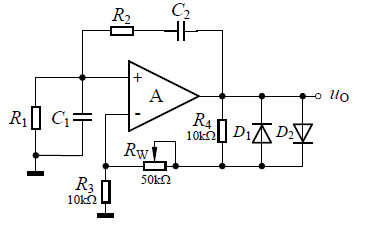
\includegraphics [width=\columnwidth]{ac.png}
\caption{正弦波发生电路}
\label{ACCirc}
\end {figure}
\end{multicols}
\subsubsection{输出波形调试}
\begin{multicols}{2}
通过调整$R_w$,我们对输出的波形进行进一步的仿真调试,如图\ref{AC0}所示,可以看到$R_w=0$的时候电路不起振,$R_w=20\%R_{max}=10\mathrm{k}\Omega$的时候电路刚好起振,如图\ref{ACstart}所示。

用示波器观测输出的波形,发现最大不失真输出电压波形大概在$R_w=40.0\%R_max=20.0\mathrm{k}\Omega$的时候取得,此时周期约为2.5ms,对应评论约为400Hz,输出电压峰值为10.35V左右,因为供电电压12v,可以看出输出性能还是很好的。对应的有效值为7.327V。输出的波形如图\ref{ACmax}所示。
\begin {figure}[H]
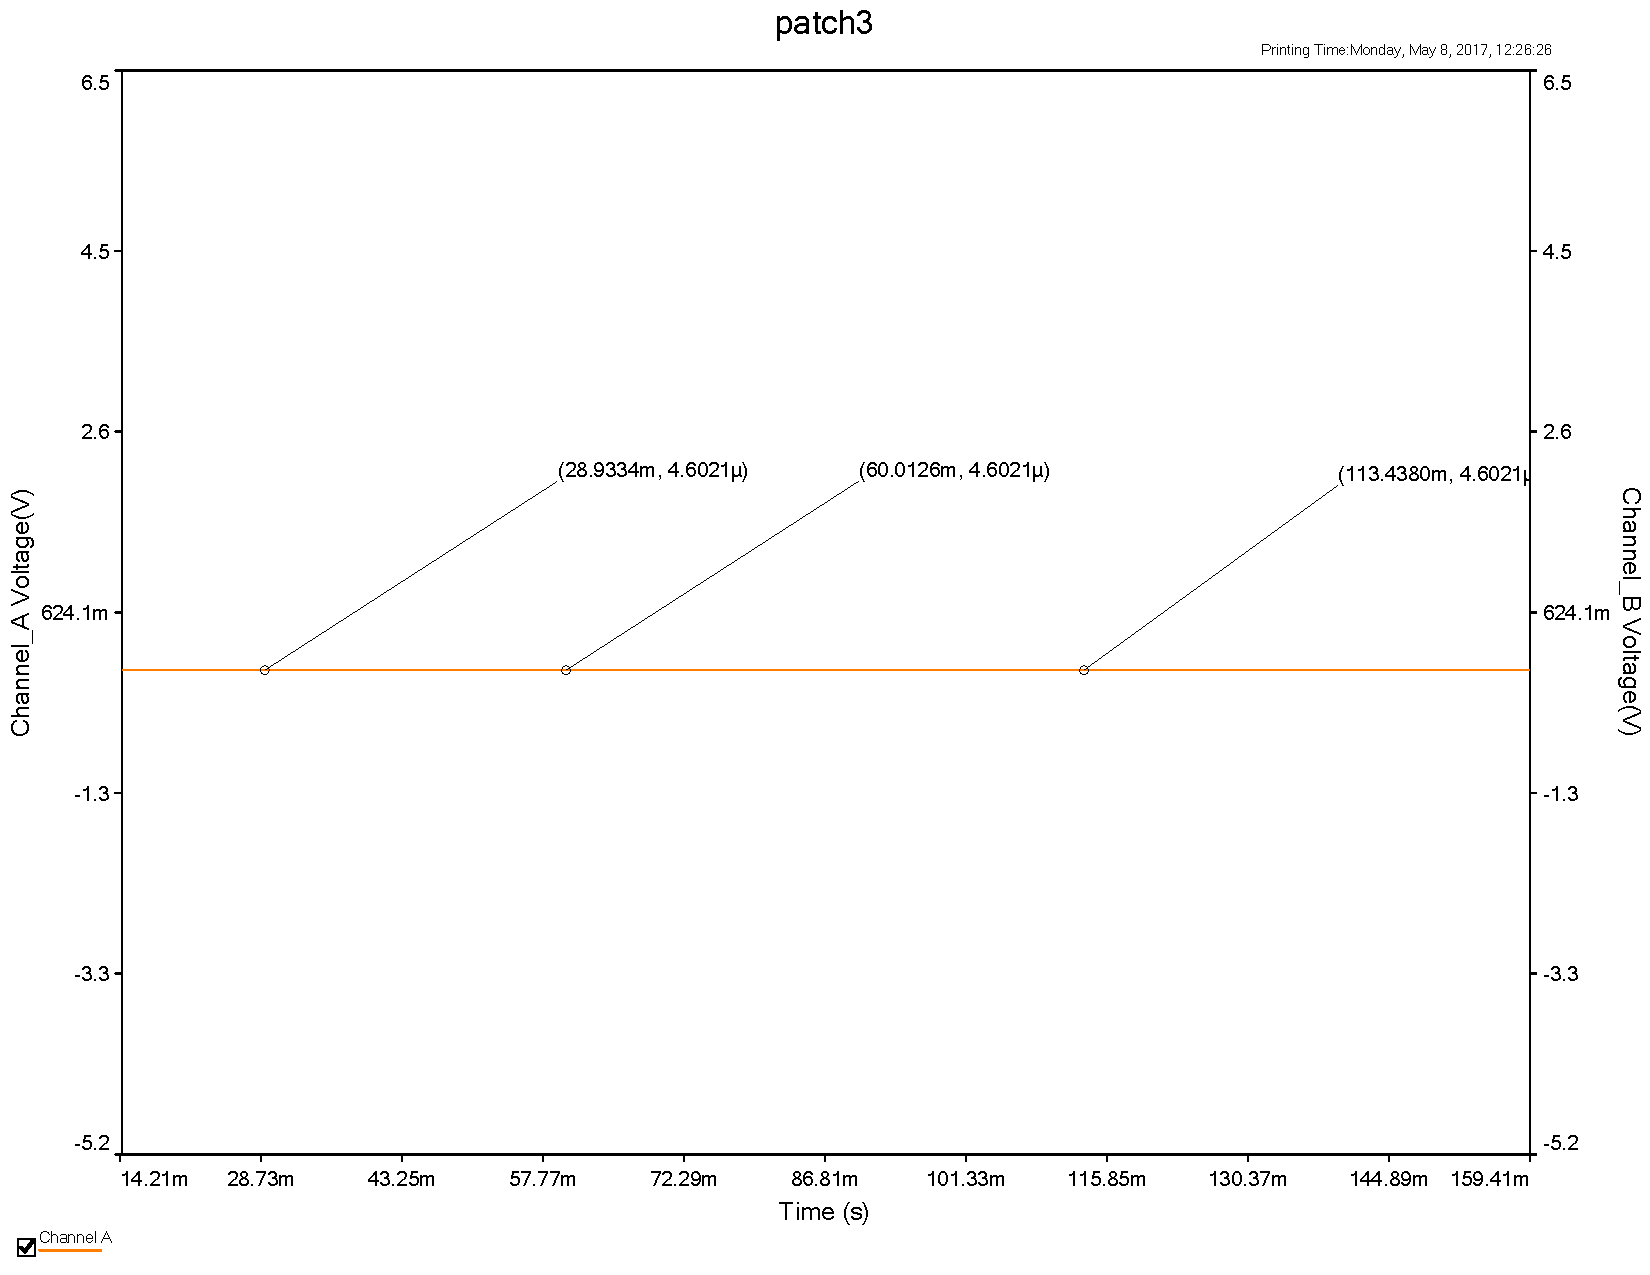
\includegraphics [width=\columnwidth]{0ac.pdf}
\caption{$R_w=0$时的输出波形}
\label{AC0}
\end {figure}
\end{multicols}
\begin{multicols}{2}
\begin {figure}[H]
\centering
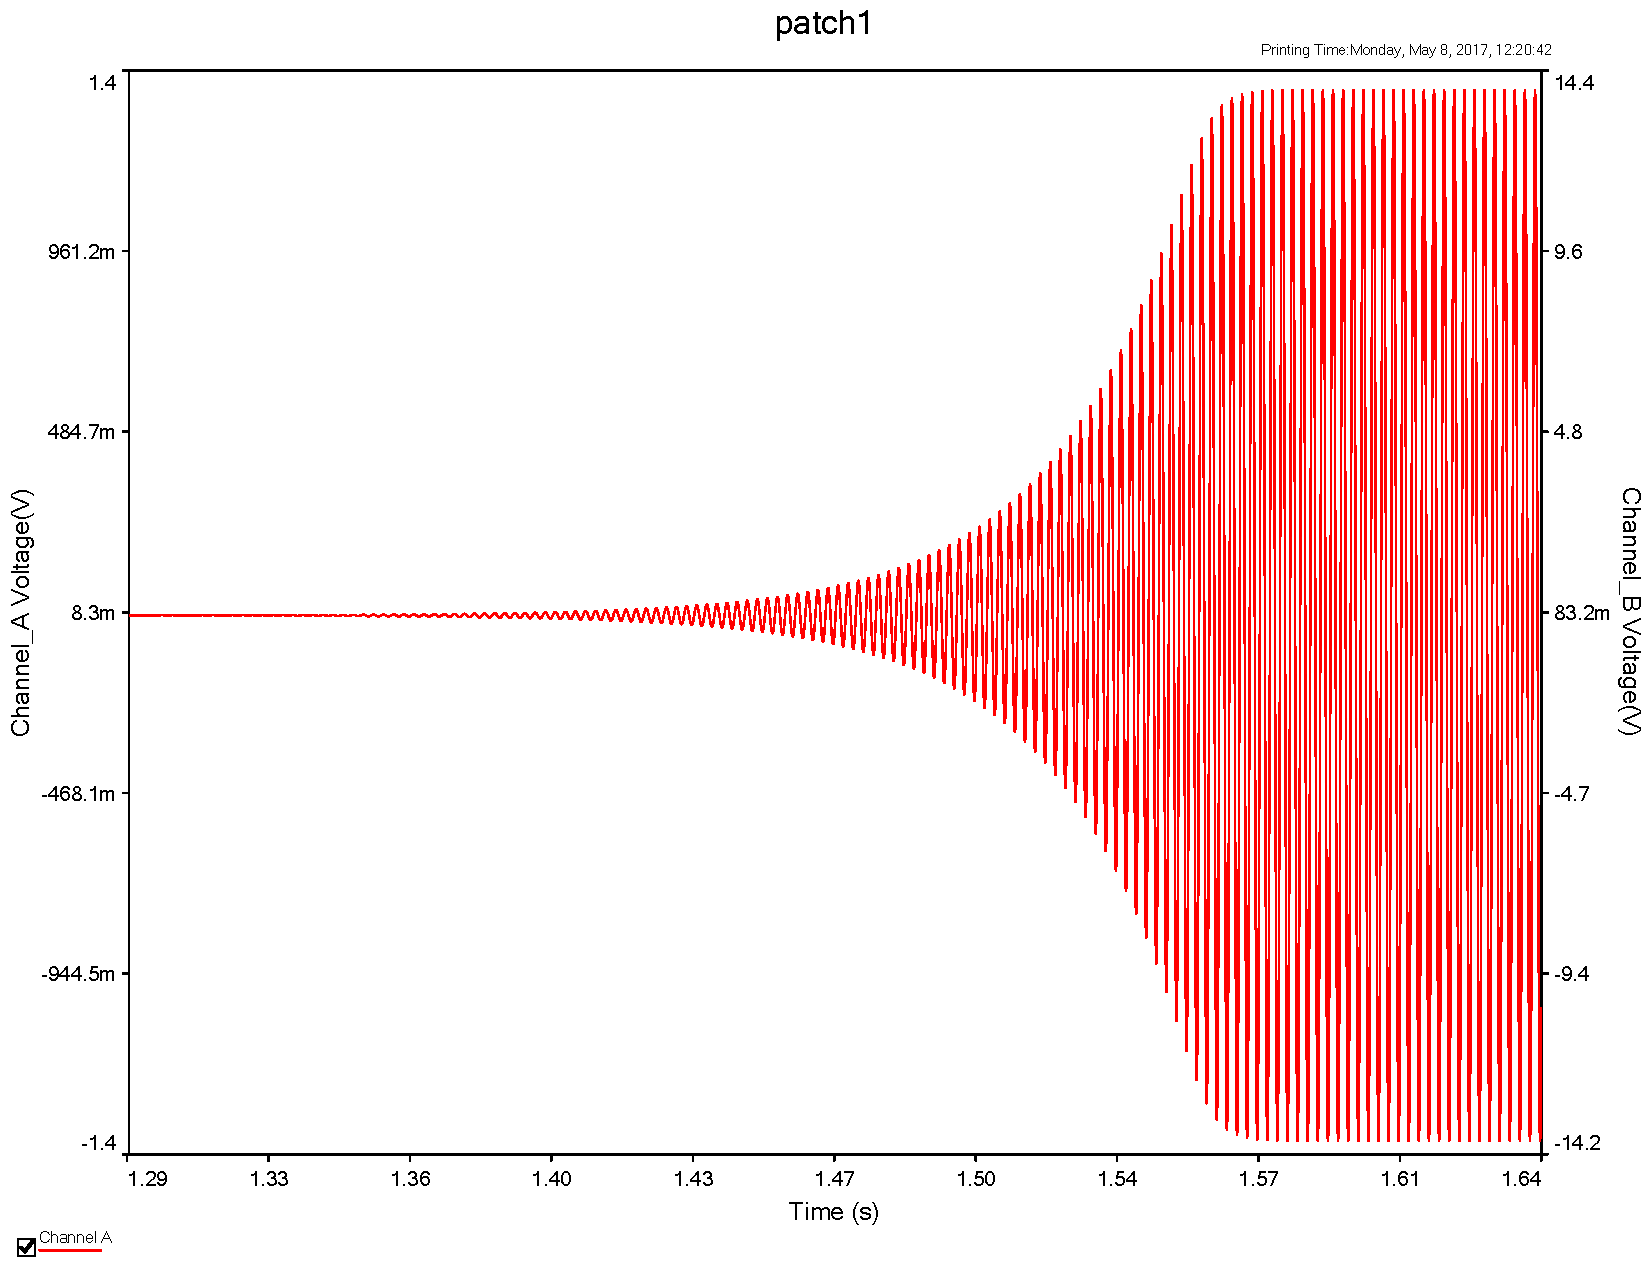
\includegraphics [width=\columnwidth]{startac.pdf}
\caption{刚刚起振输出波形}
\label{ACstart}
\end {figure}
\begin{figure}[H]
\centering
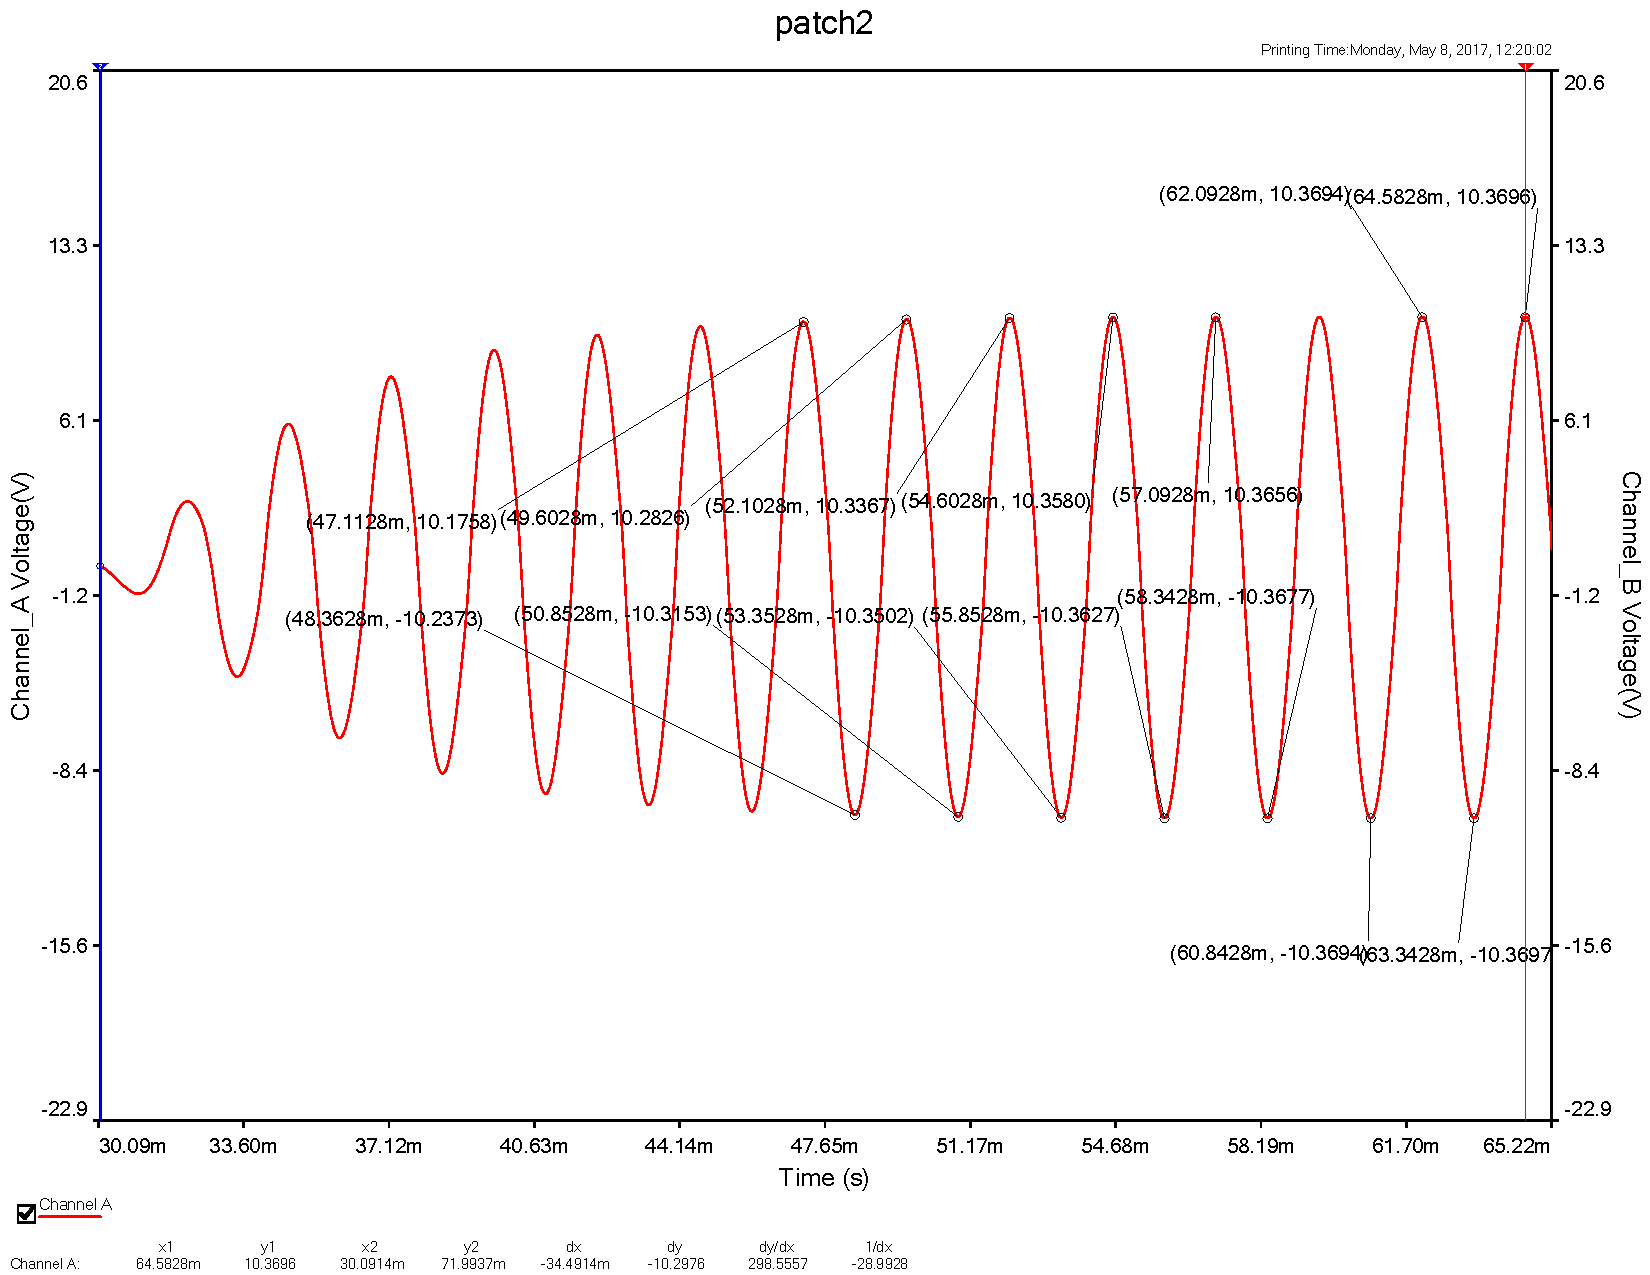
\includegraphics[width=\columnwidth]{maxac.pdf}
\caption{输出最大不失真波形}
\label{ACmax}
\end{figure}
\end{multicols}
\subsubsection{其他情况的调试}
将两个二极管断开,$R_w$从小到大变化时,输出波形的变化情况如图\ref{20}-\ref{infi}所示,可以总结为如下几点
\begin{enumerate}
\item $R_w < 10 \mathrm{k}\Omega$时,无法产生震荡
\item $R_w > 10 \mathrm{k}\Omega$时,输出一直缓慢增大到最大不失真电压
\item 随着$R_w$的明显增大,输出波形失真变得越来越明显,越来越趋近于方波,方波的上升时间和下降时间逐渐减小。
\end{enumerate}
\begin{multicols}{2}
\begin{figure}[H]
\centering
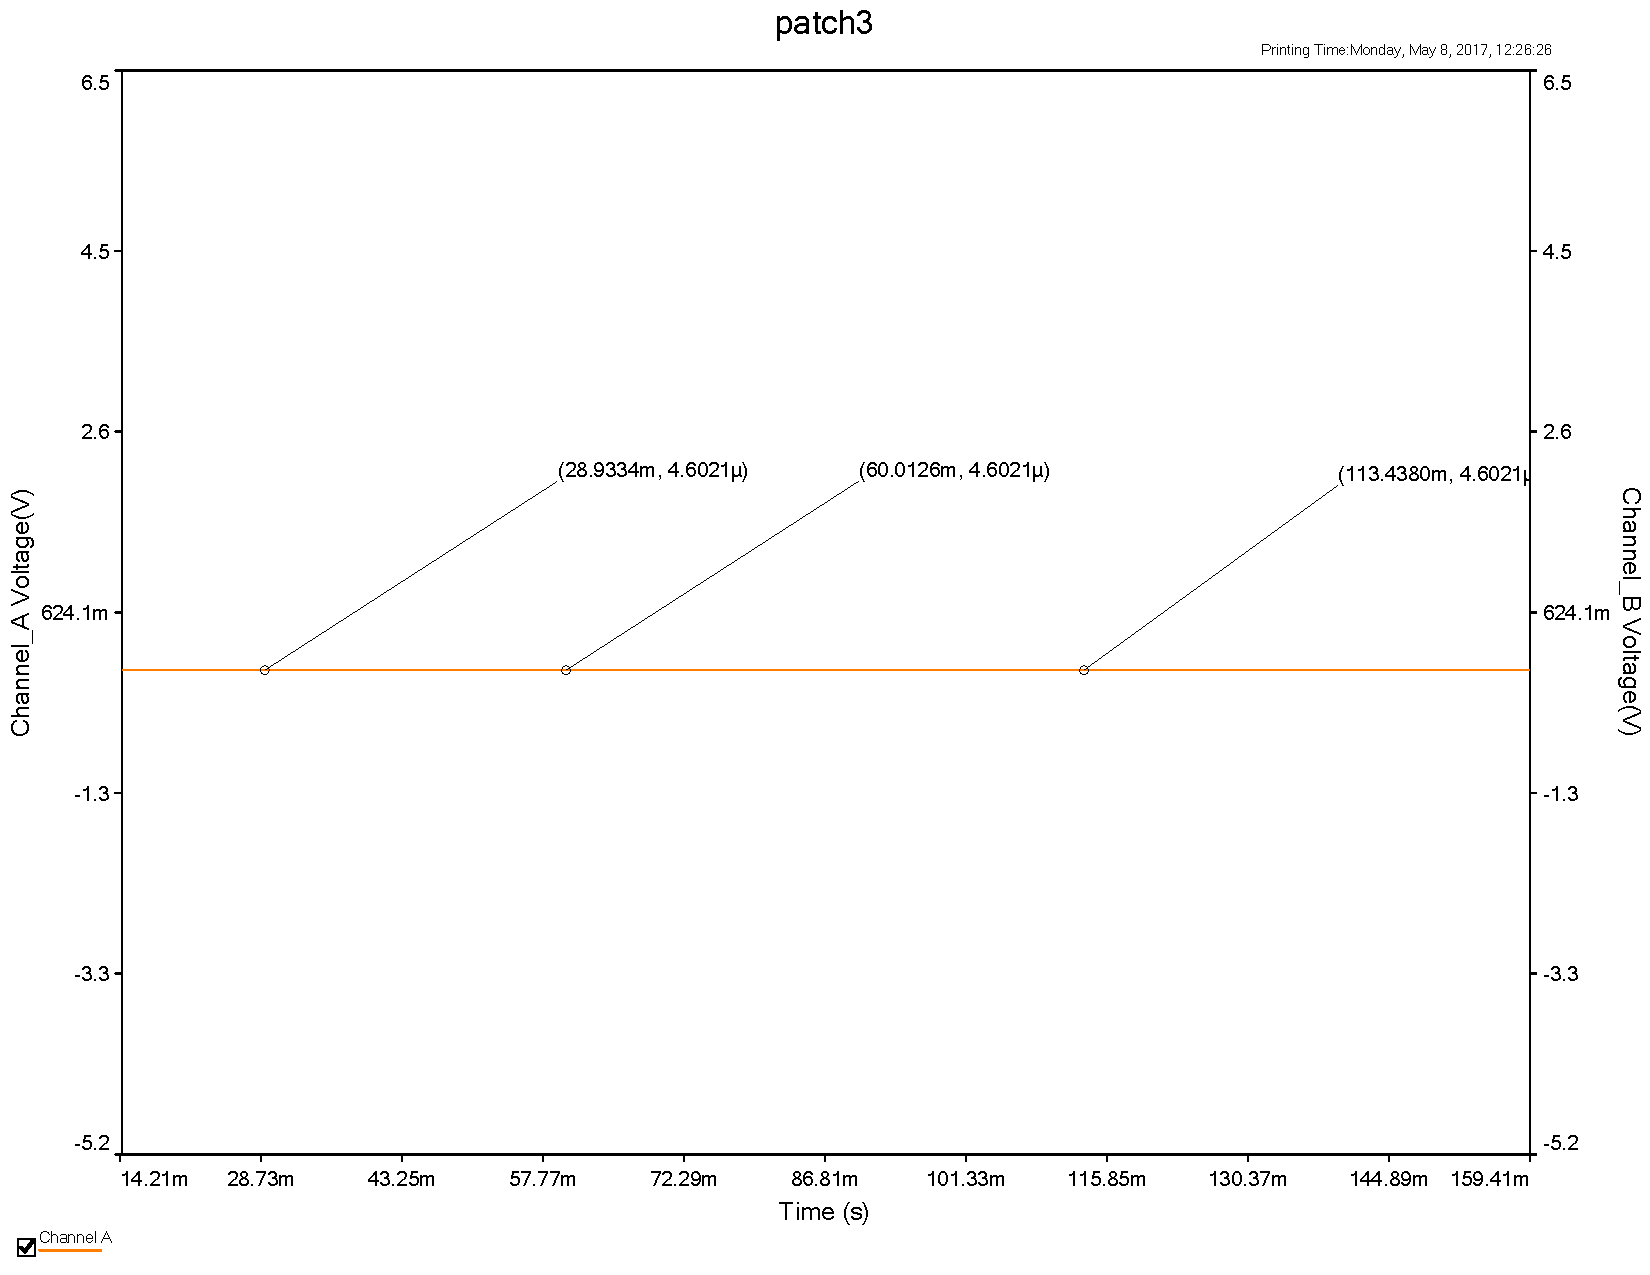
\includegraphics[width=\columnwidth]{0ac.pdf}
\caption{$R_w=20\%$时的输出波形}
\label{20}
\end{figure}
\begin{figure}[H]
\centering
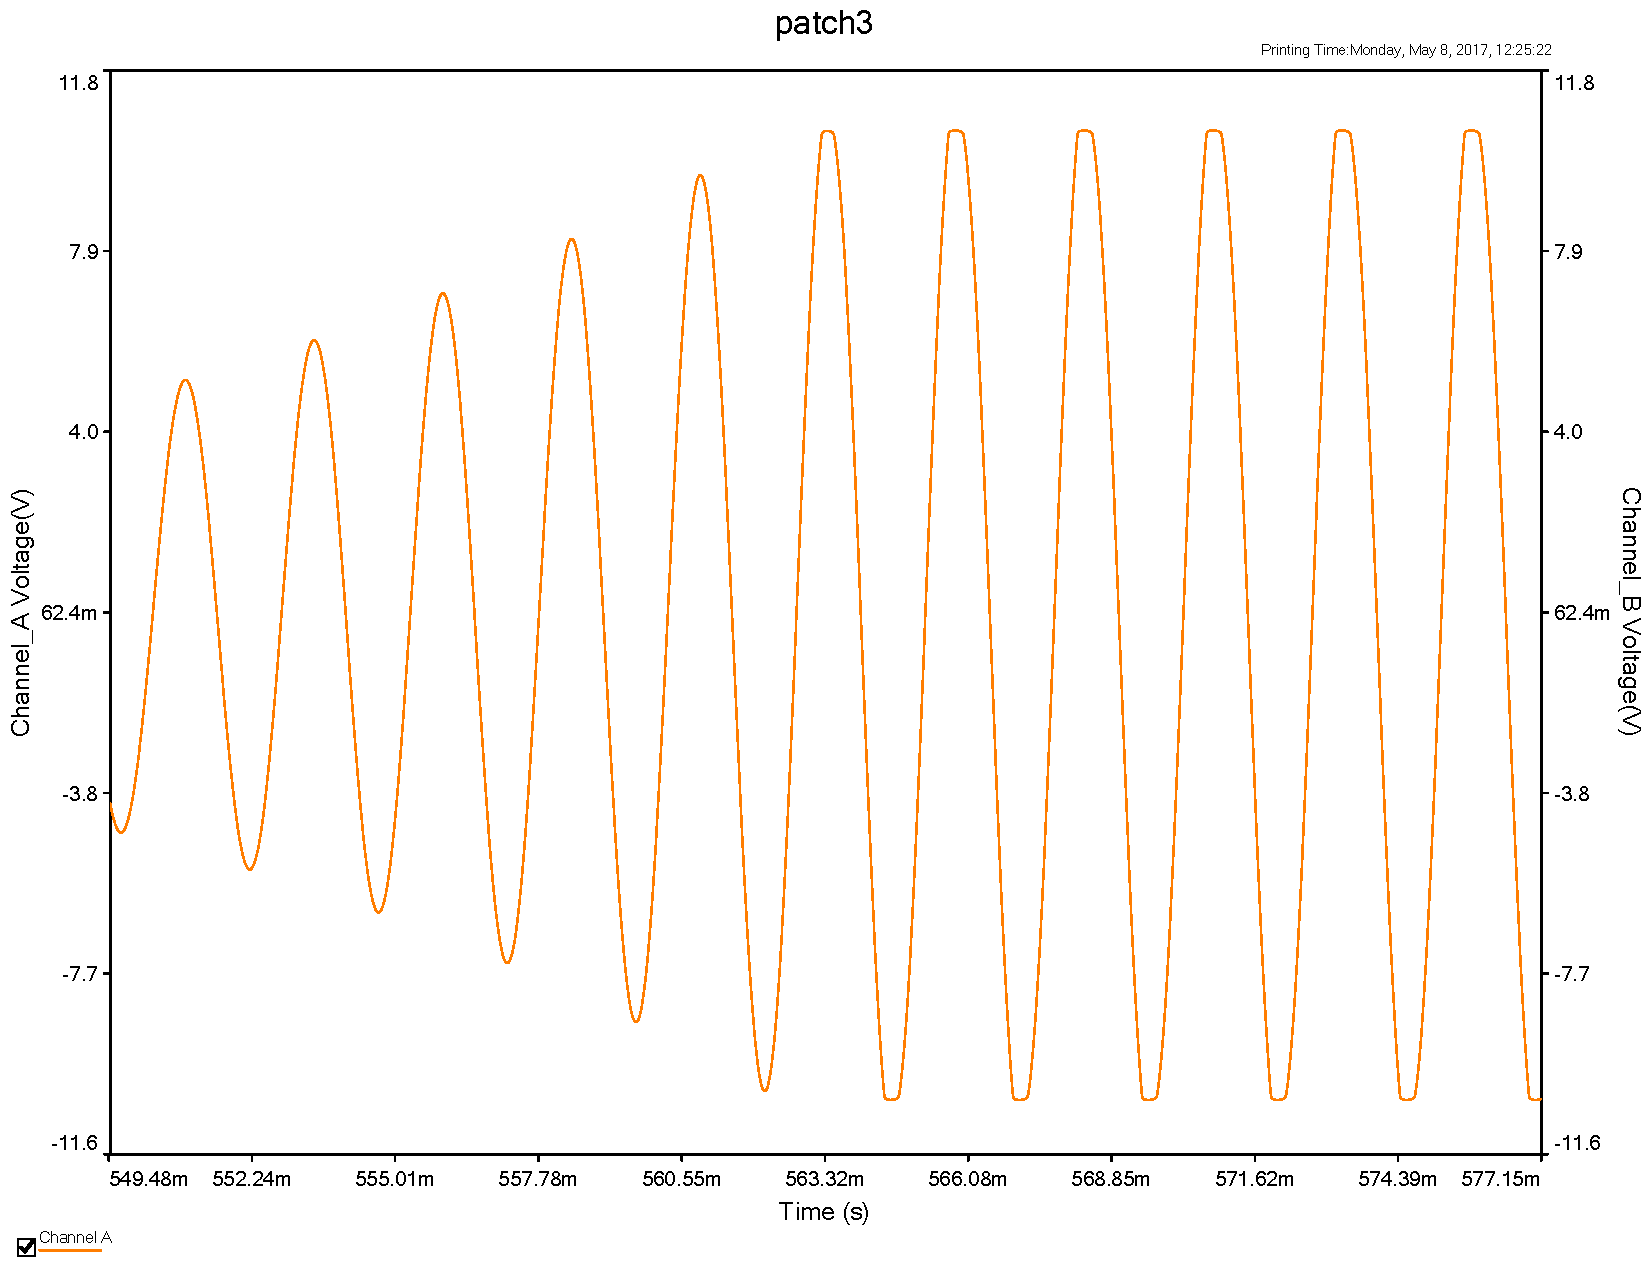
\includegraphics[width=\columnwidth]{21ac.pdf}
\caption{$R_w=21\%$时的输出波形}
\label{21}
\end{figure}
\begin{figure}[H]
\centering
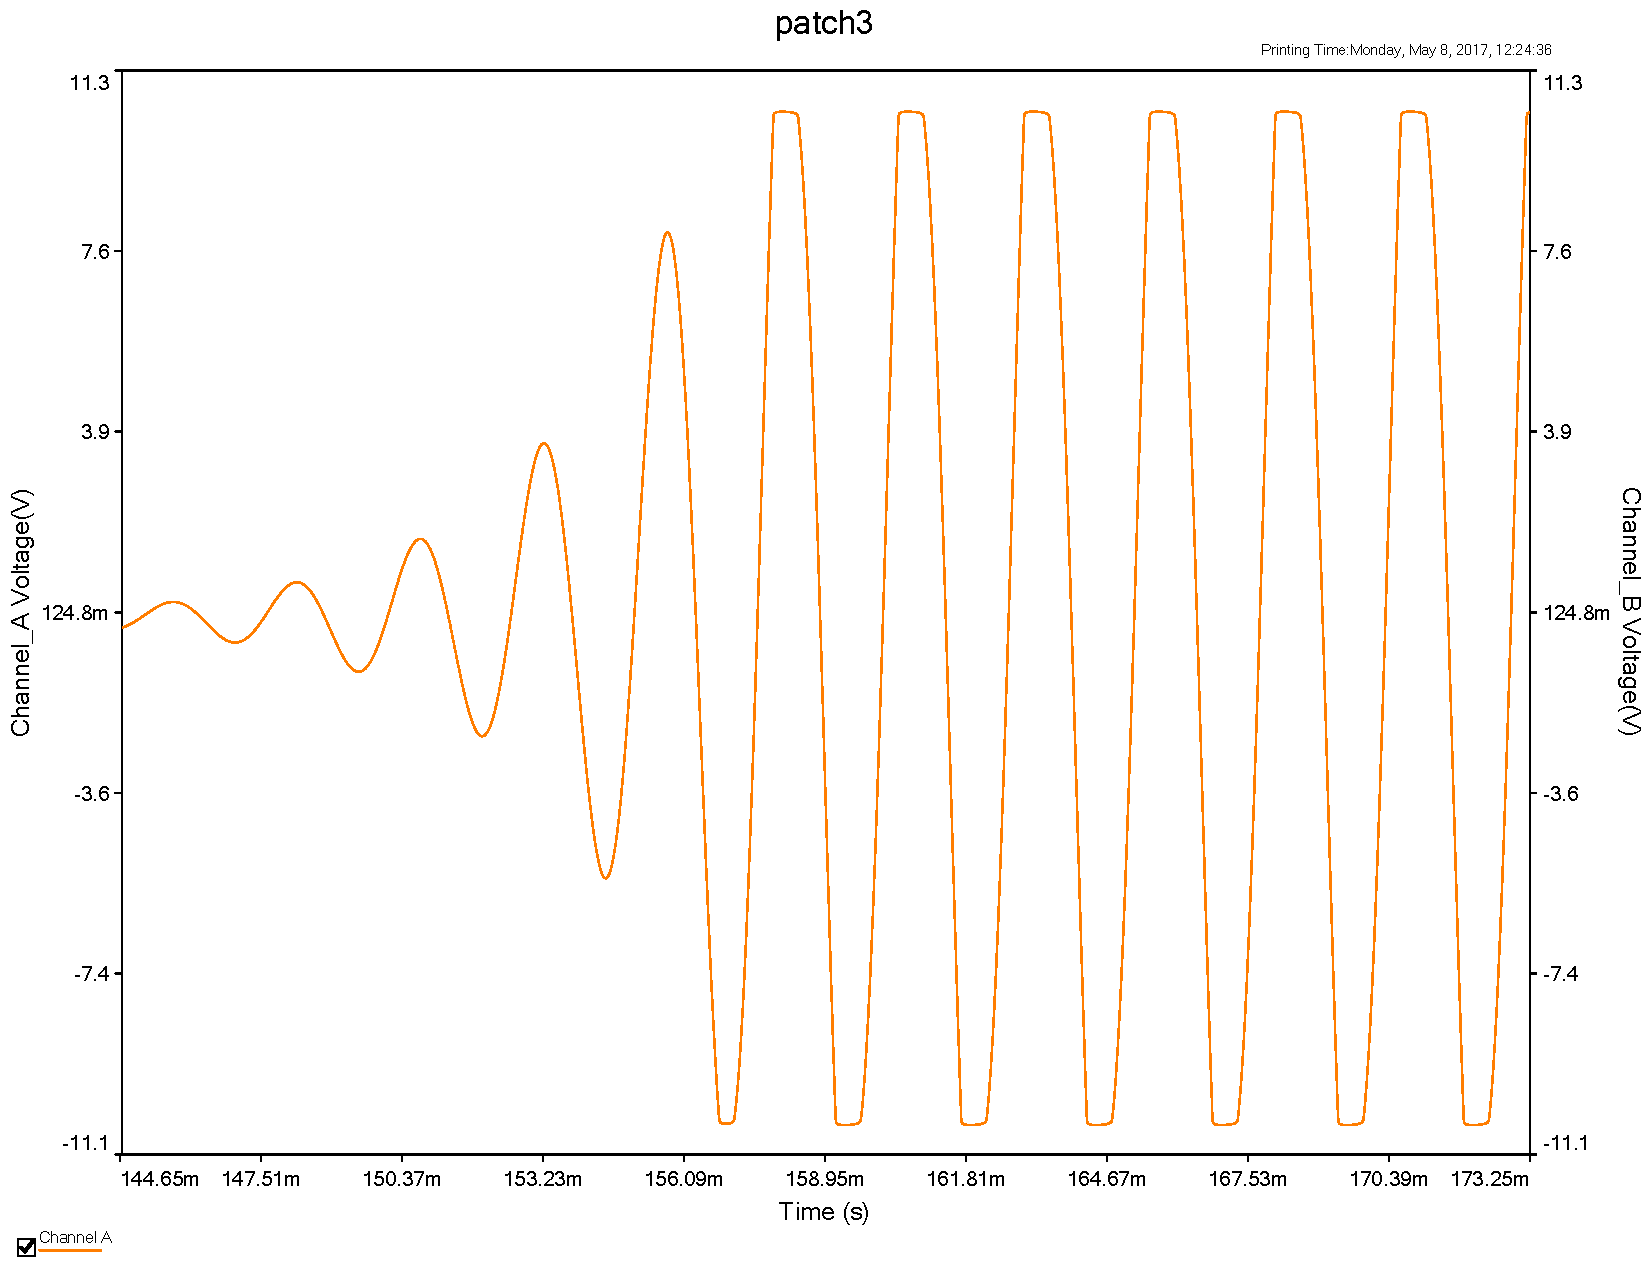
\includegraphics[width=\columnwidth]{25ac.pdf}
\caption{$R_w=25\%$时的输出波形}
\label{25}
\end{figure}
\begin{figure}[H]
\centering
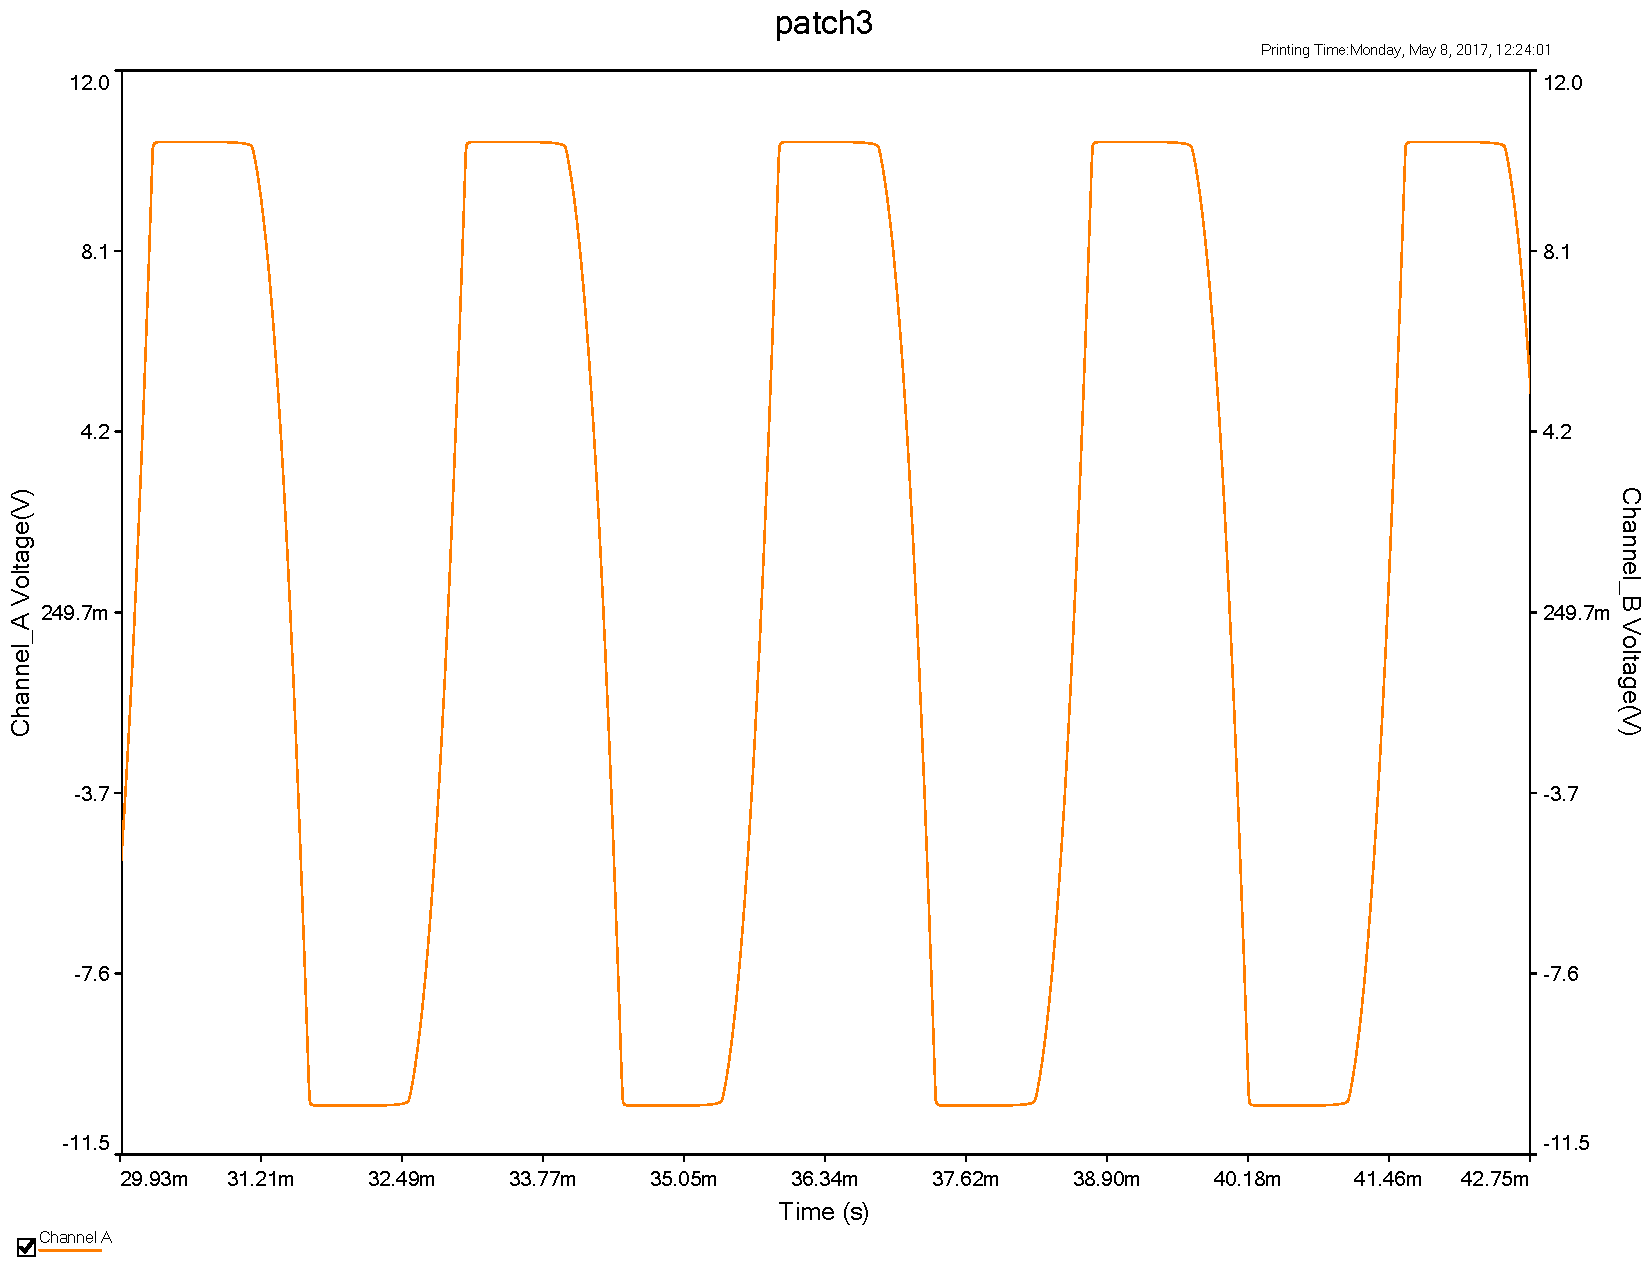
\includegraphics[width=\columnwidth]{40ac.pdf}
\caption{$R_w=40\%$时的输出波形}
\label{40}
\end{figure}
\begin{figure}[H]
\centering
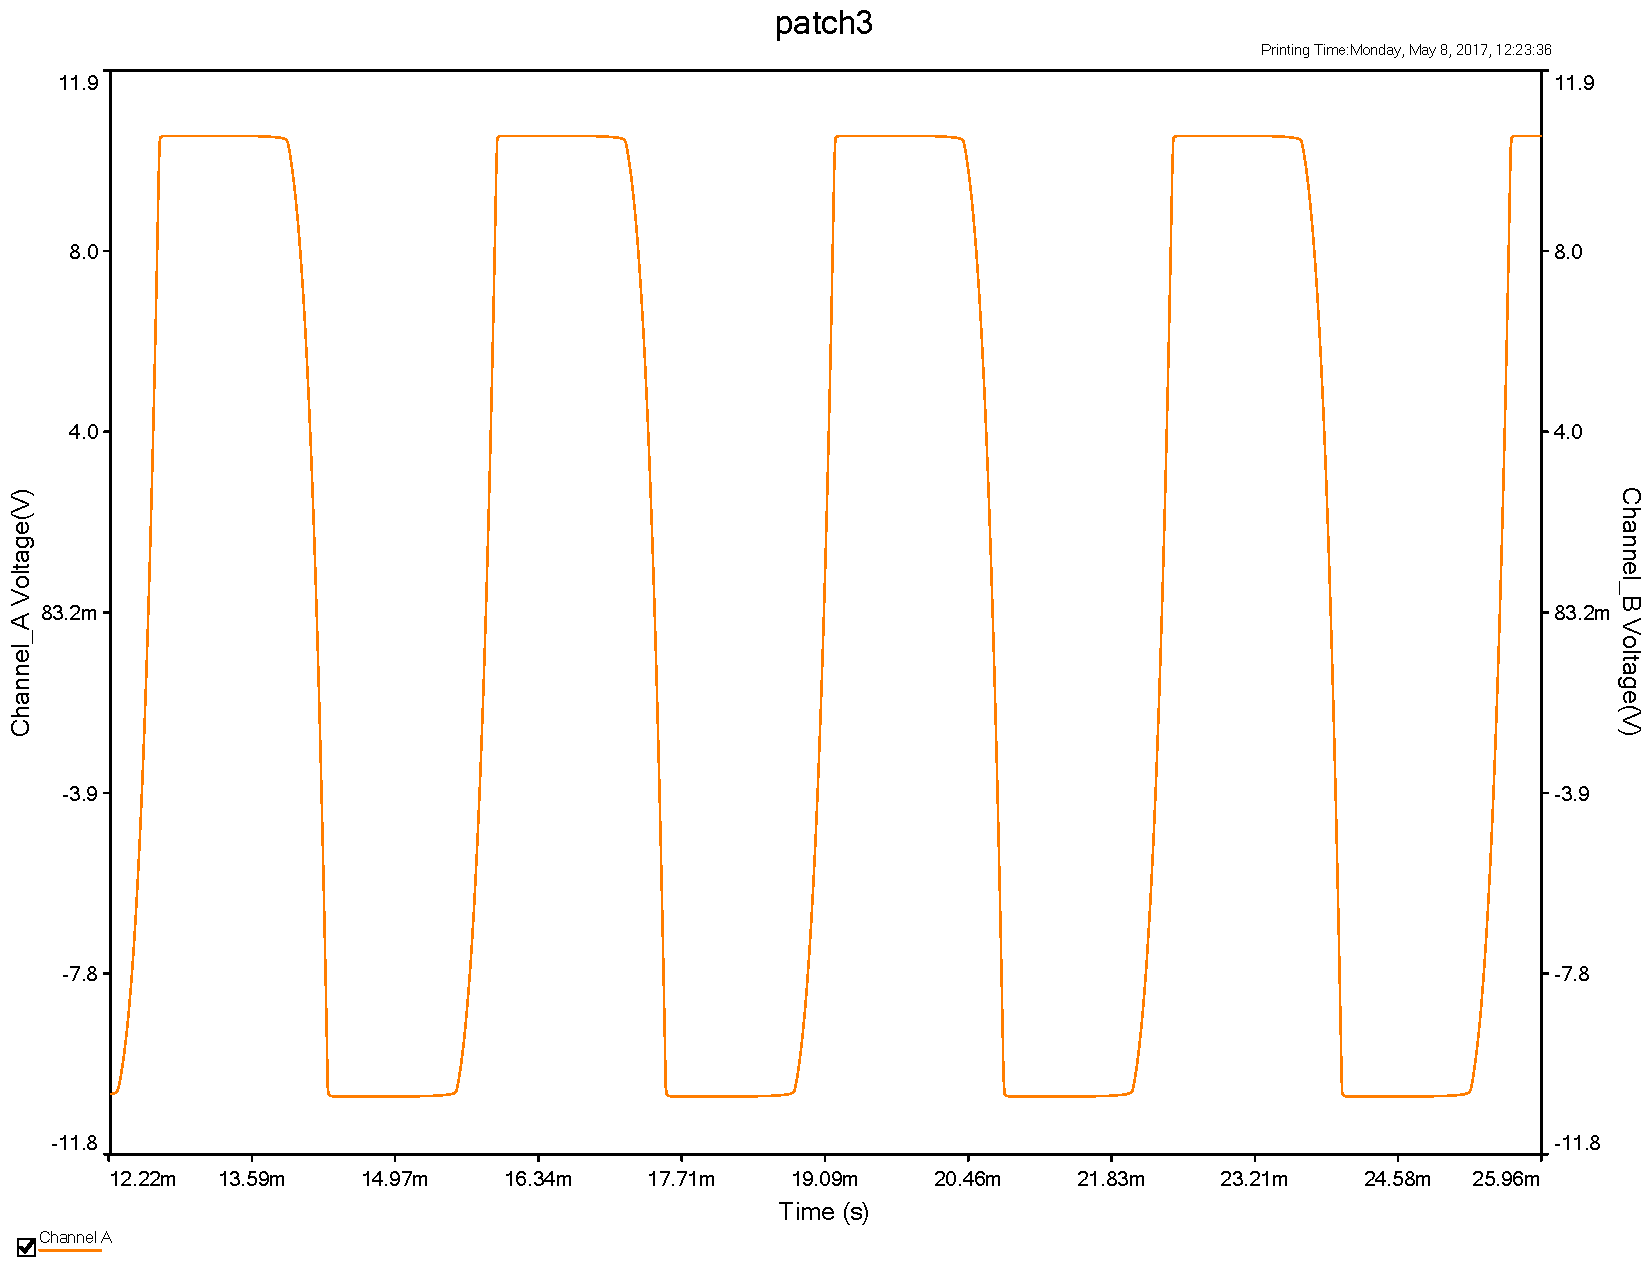
\includegraphics[width=\columnwidth]{60ac.pdf}
\caption{$R_w=60\%$时的输出波形}
\label{60}
\end{figure}
\begin{figure}[H]
\centering
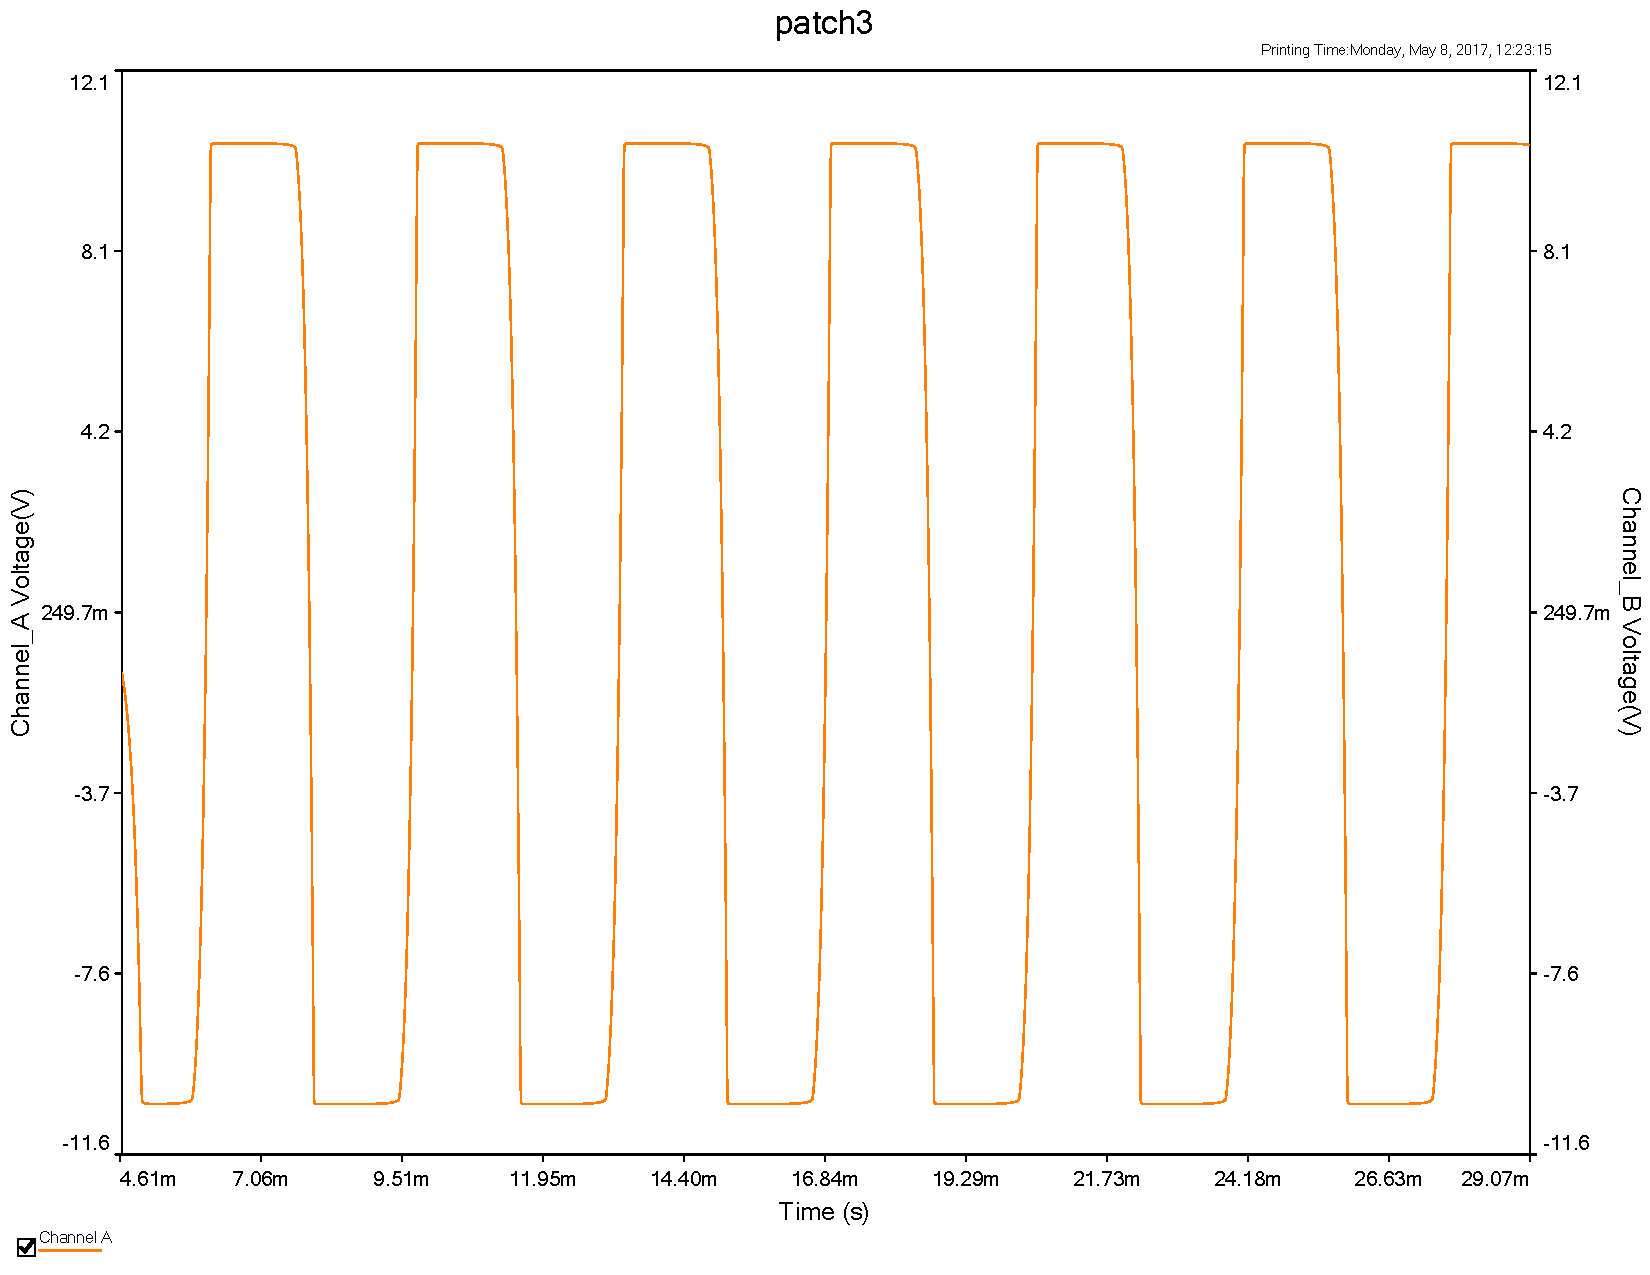
\includegraphics[width=\columnwidth]{80ac.pdf}
\caption{$R_w=80\%$时的输出波形}
\label{80}
\end{figure}
\begin{figure}[H]
\centering
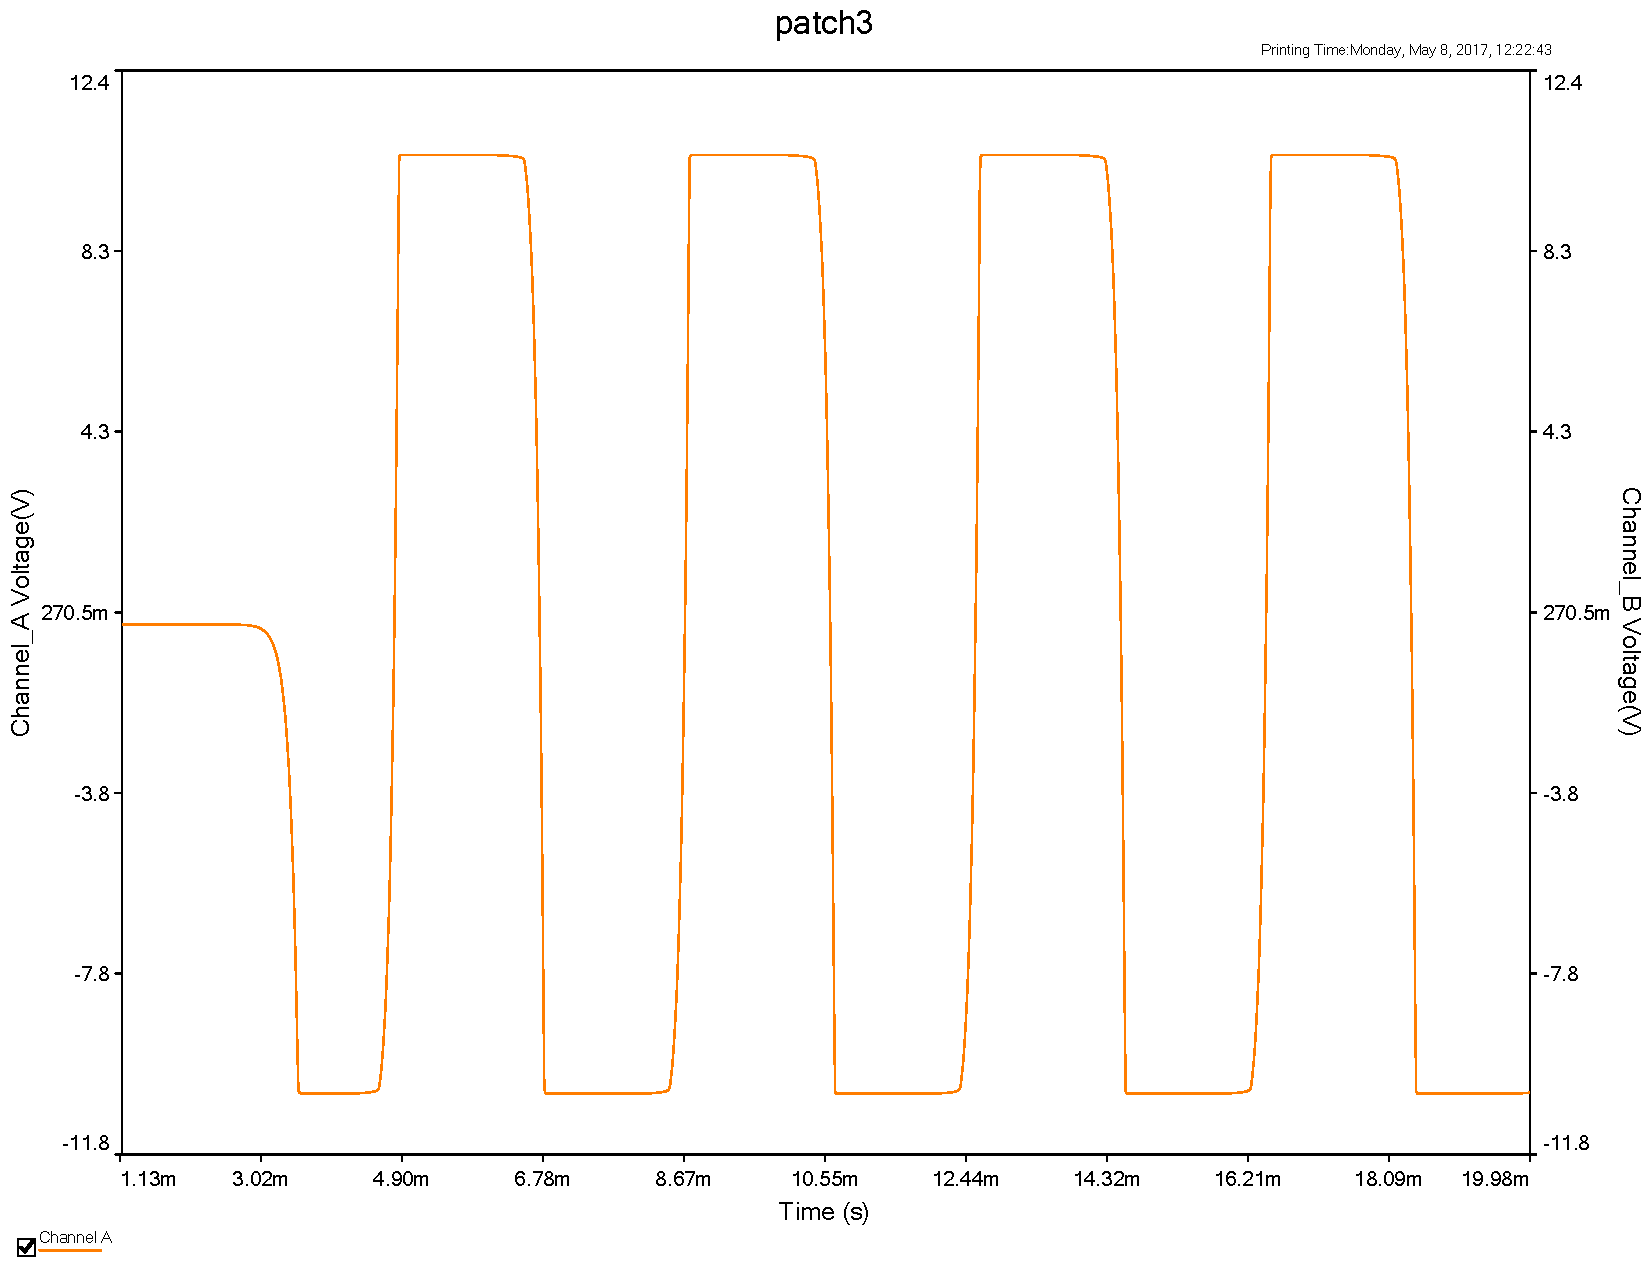
\includegraphics[width=\columnwidth]{100ac.pdf}
\caption{$R_w=100\%$时的输出波形}
\label{100}
\end{figure}
\begin{figure}[H]
\centering
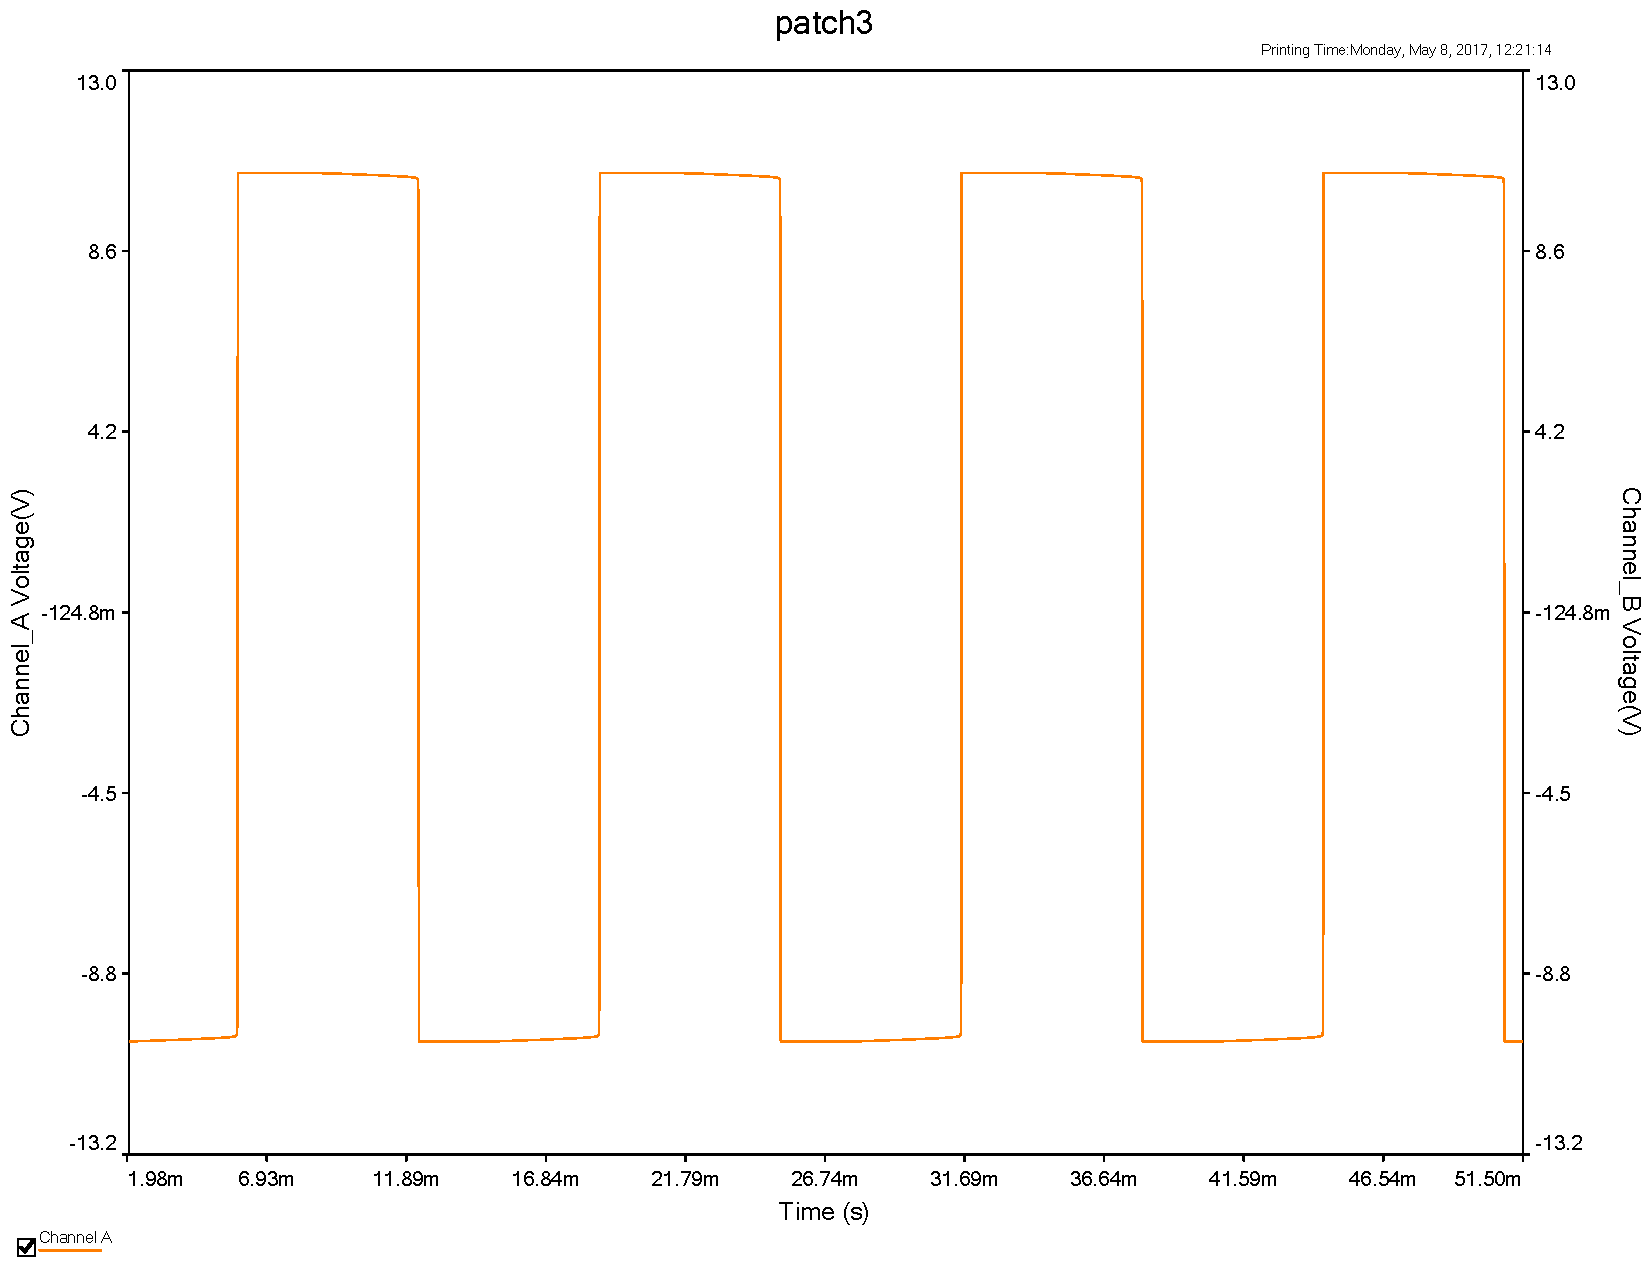
\includegraphics[width=\columnwidth]{offac.pdf}
\caption{$R_w$完全断开时的输出波形}
\label{infi}
\end{figure}
\end{multicols}
\subsection{方波——三角波发生电路}
\subsubsection{理论分析}
\label{sec:}
\begin{multicols}{2}
如图\ref{BICirc}是方波——三角波发生电路的电路图

首先对电路进行理论估计,为了和实验值保持一致,改用了和实验室提供的稳压管相同导通压降$U_Z=5.1\mathrm{V}$的稳压管1N4733A,得到左侧同相输入滞环特性的阈值电压方程
$$\frac{R_1}{R_1+R_2}U_T\pm\frac{R_2}{R_1+R_2}U_Z=0$$
得到
$$U_T=\pm\frac{R_2}{R_1}U_Z=2.55\mathrm{V}$$
右侧电路为积分运算电路,输出电压的表达式为
$$U_0=\int U_Z\mathrm{d}t$$半个周期内积分从$-U_T$抵达$+U_T$,因此可以得到$$2U_T=\frac{T}{2}\frac{U_Z}{R_4C}$$结合前几式可以得到$$T=\frac{4R_2R_4C}{R_1}=0.4\mathrm{mS}$$
\begin {figure}[H]
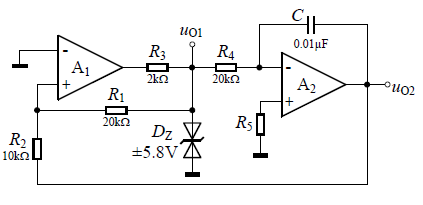
\includegraphics [width=\columnwidth]{bi.png}
\caption{方波——三角波发生电路}
\label{BICirc}
\end {figure}
\end{multicols}
\subsubsection{波形仿真}
从图\ref{BI}所示我们可以看到方波——三角波电路的产生过程,我们可以看到方波的幅值大约为5.5313V,而三角波的幅值为2.6018V,三角波的对称性良好,两个信号的周期为0.4076ms,和理论计算基本相符,上升时间和下降时间均为0.2038ms。
\begin{figure}
\centering
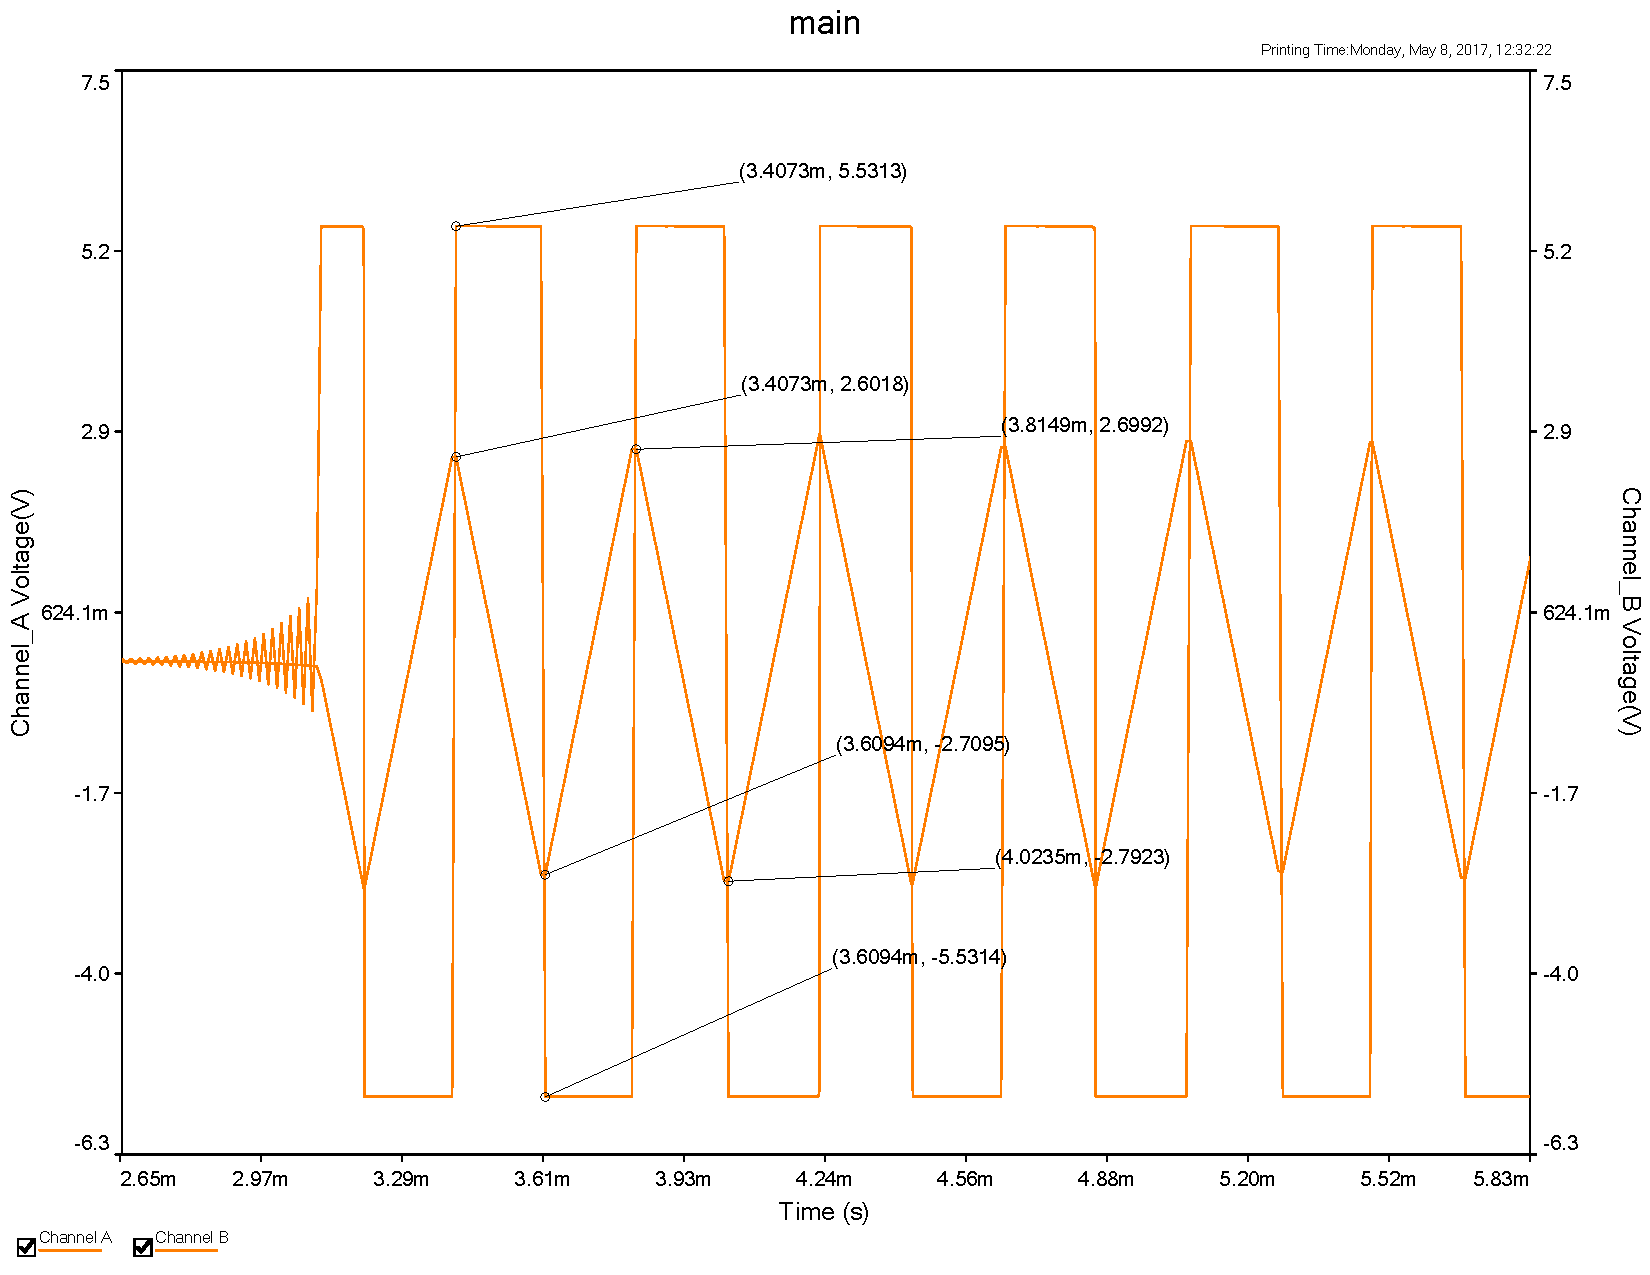
\includegraphics[width=\textwidth]{bi.pdf}
\caption{方波——三角波发生电路输出波形}
\label{BI}
\end{figure}
\subsection{滞环特性电路的测试}
\subsubsection{理论分析}
如图\ref{schiCrit}是滞环特性电路电路图,有关$U_T$的推导的问题可以参阅\ref{sec:}节的说明,这里就不加重复了。
\begin {figure}
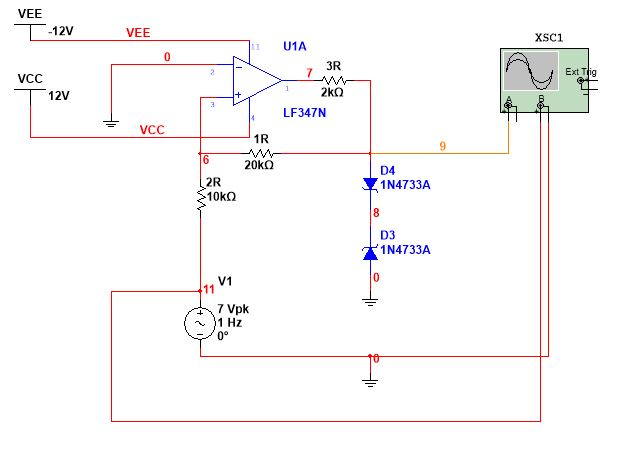
\includegraphics [width=\textwidth]{sch.jpg}
\caption{滞环特性电路}
\label{schiCrit}
\end {figure}
\subsubsection{输出波形仿真}
从图\ref{sch}可以看出滞环特性仿真电路,可以看出电路的$U_T=\pm 2.718\mathrm{V}$,输出电压为$U_O=\pm 5.5382\mathrm{V}$,滞环特性曲线形状良好。
\begin{figure}
\centering
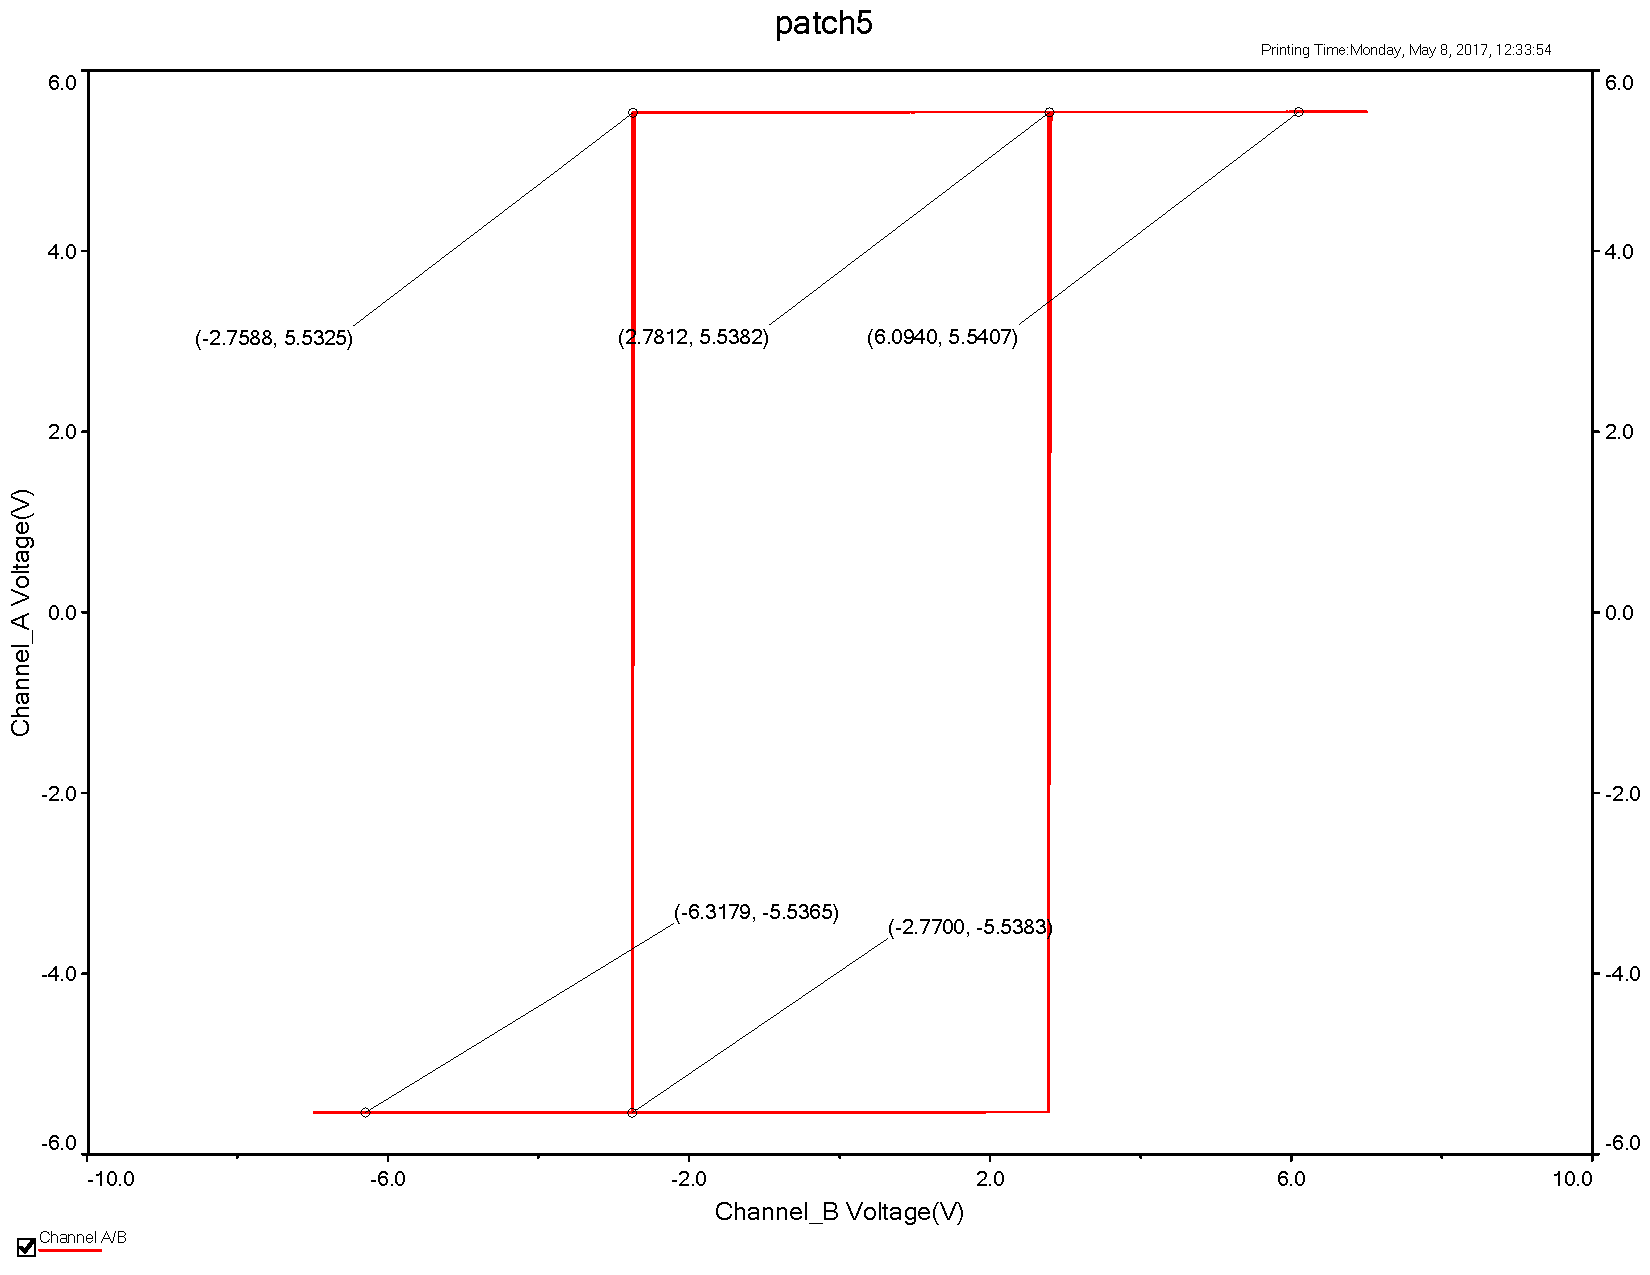
\includegraphics[width=\textwidth]{sch.pdf}
\caption{滞环特性输出波形}
\label{sch}
\end{figure}
\subsection{锯齿波发生电路}
\subsubsection{理论分析}
如图\ref{tanCrit}所示是锯齿波发生电路的测试图,根据\ref{sec:}一节的说明,我们设两个二极管的正向导通电压降为$U_D$,可以根据电路图可以得到上升和下降的方程($R_1,R_2$位置见图所示)
$$2U_T=T_-\frac{U_Z-U_D}{R_1C}$$
$$2U_T=T_+\frac{U_Z-U_D}{R_2C}$$
因此可以得到上升沿和下降沿时间
$$T_-=\frac{2U_TR_1C}{U_Z-U_D}$$
$$T_+=\frac{2U_TR_2C}{U_Z-U_D}$$
需要锯齿波下降时间为上升时间的20\%马上得到$5R_1=R_2$

同时要求电路周期不变,得到$$\frac{2U_T(R_1+R_2)C}{U_Z-U_D}=0.4\mathrm{mS}$$
可以迅速解得$R_1=5.816\mathrm{k}\Omega$,进一步得到$R_2=29.084\mathrm{k}\Omega$

具体选取$R_1=6\mathrm{k}\Omega,R_2=30\mathrm{k}\Omega$
\begin {figure}
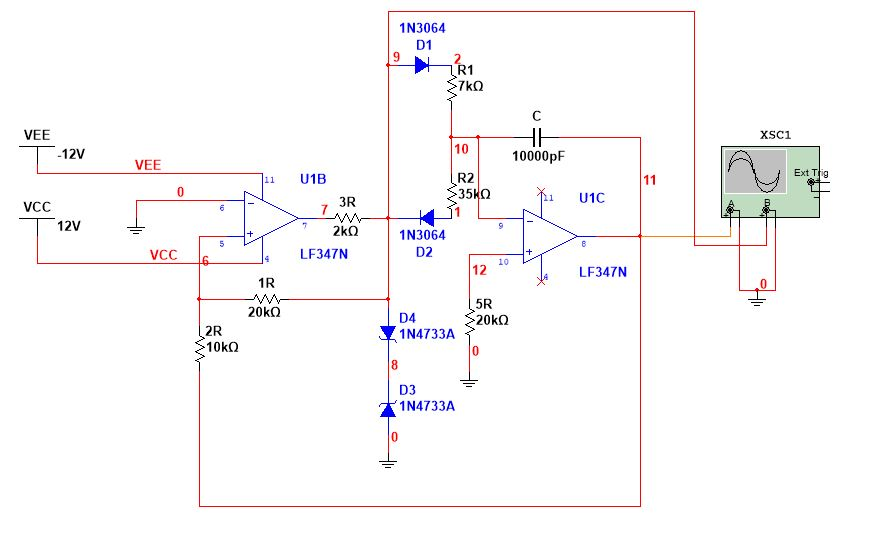
\includegraphics [width=\textwidth]{tan.jpg}
\caption{锯齿波发生电路}
\label{tanCrit}
\end {figure}
\begin{multicols}{2}
\subsubsection{输出波形仿真}
从图\ref{tan}中我们可以看到,方波和锯齿波的0.10周期均为0.4315ms,这种变化源自于电阻取整之后引入的误差,锯齿波的上升时间为0.3222ms,下降时间为0.1093ms,下降时间和上升时间的比值稍大,考虑是电阻取整的影响,将电阻取值改变为$7\mathrm{k}\Omega$和$35\mathrm{k}\Omega$发现电路性能出现明显好转。
\begin{figure}[H]
\centering
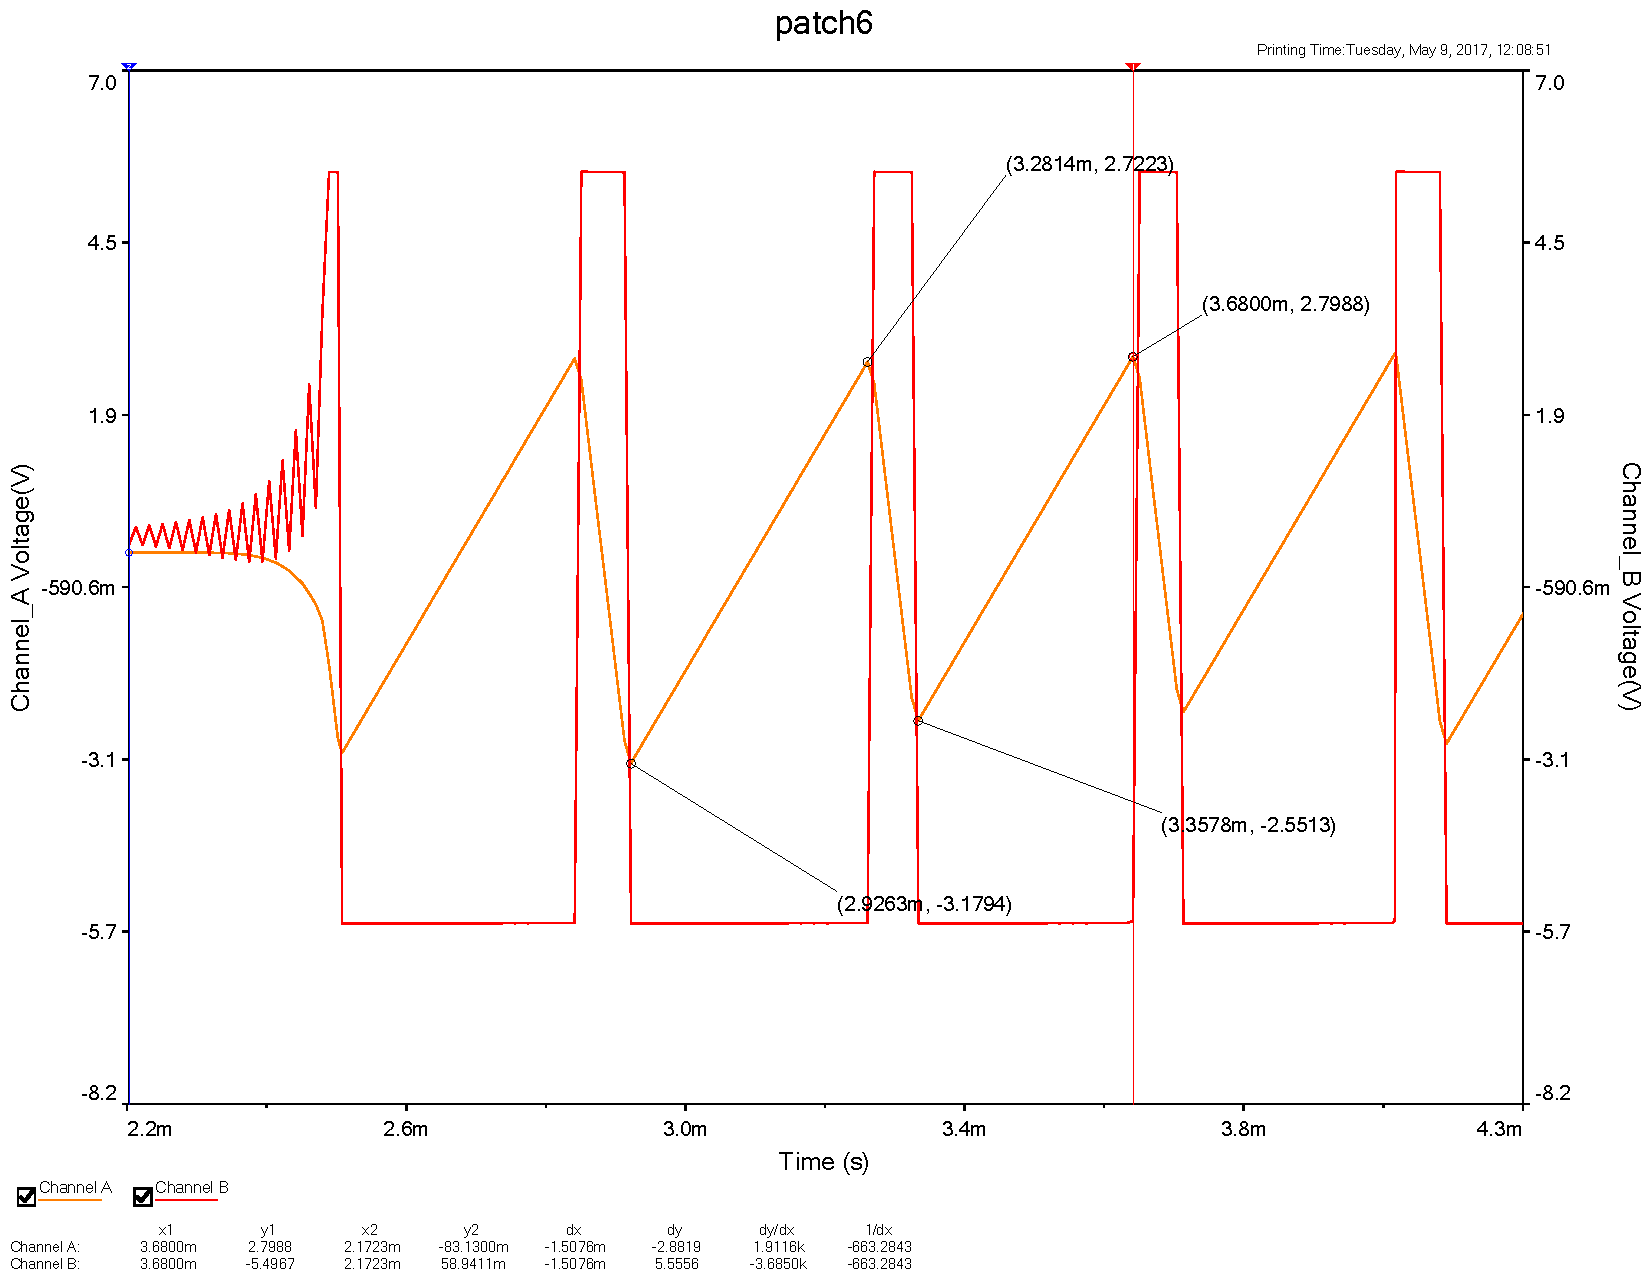
\includegraphics[width=\columnwidth]{tan.pdf}
\caption{锯齿波发生电路输出波形}
\label{tan}
\end{figure}
\end{multicols}
\clearpage
\section{实验数据记录}
\begin{multicols}{2}
\subsection{正弦波发生电路}
实验测得在$R_w=9.3\mathrm{k}\Omega$时电路起振,起振正弦波峰峰值为$V_{pp}=540\mathrm{mV}$,对应频率为416Hz。
\begin{figure}[H]
\centering
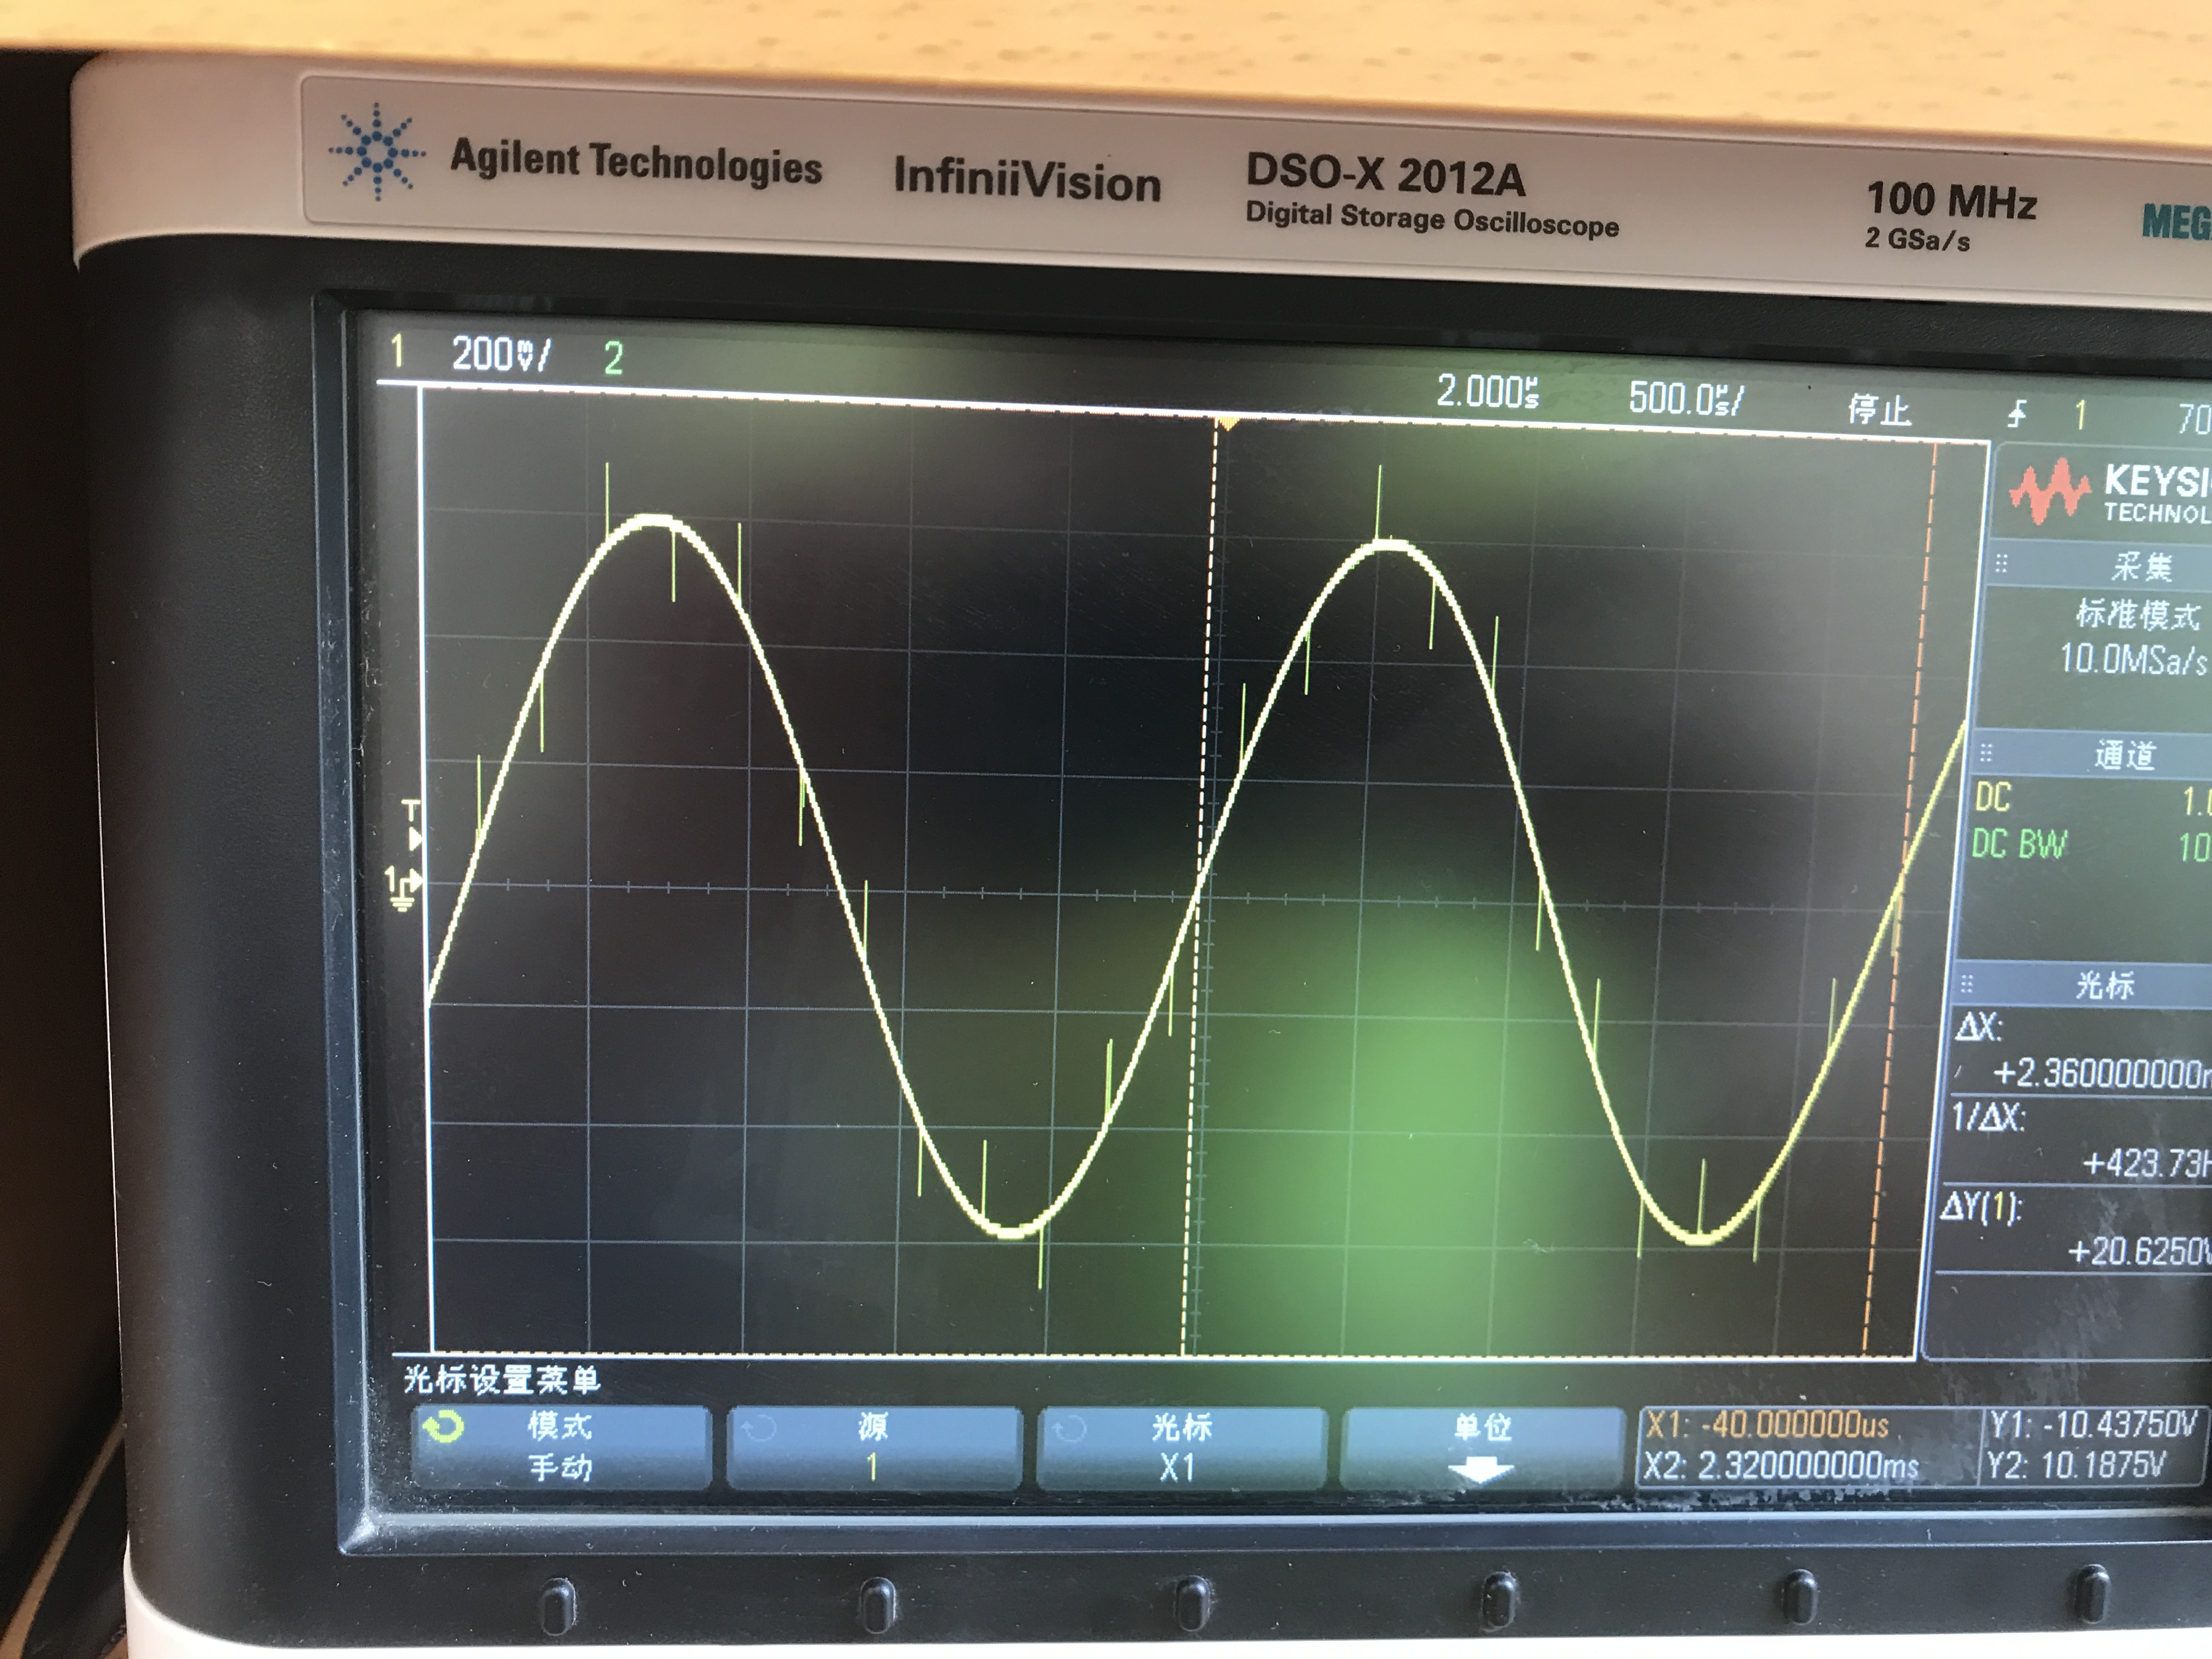
\includegraphics[width=\columnwidth,angle=0]{wave/IMG_0635.jpg}
\caption{刚刚起振输出波形}
\label{1}
\end{figure}
\end{multicols}
\begin{multicols}{2}
当$R_w=17.69\mathrm{k}\Omega$时电路出现最大不失真输出电压,峰峰值为$V_{pp}=20.62\mathrm{V}$,对应频率为423Hz
\begin{figure}[H]
\centering
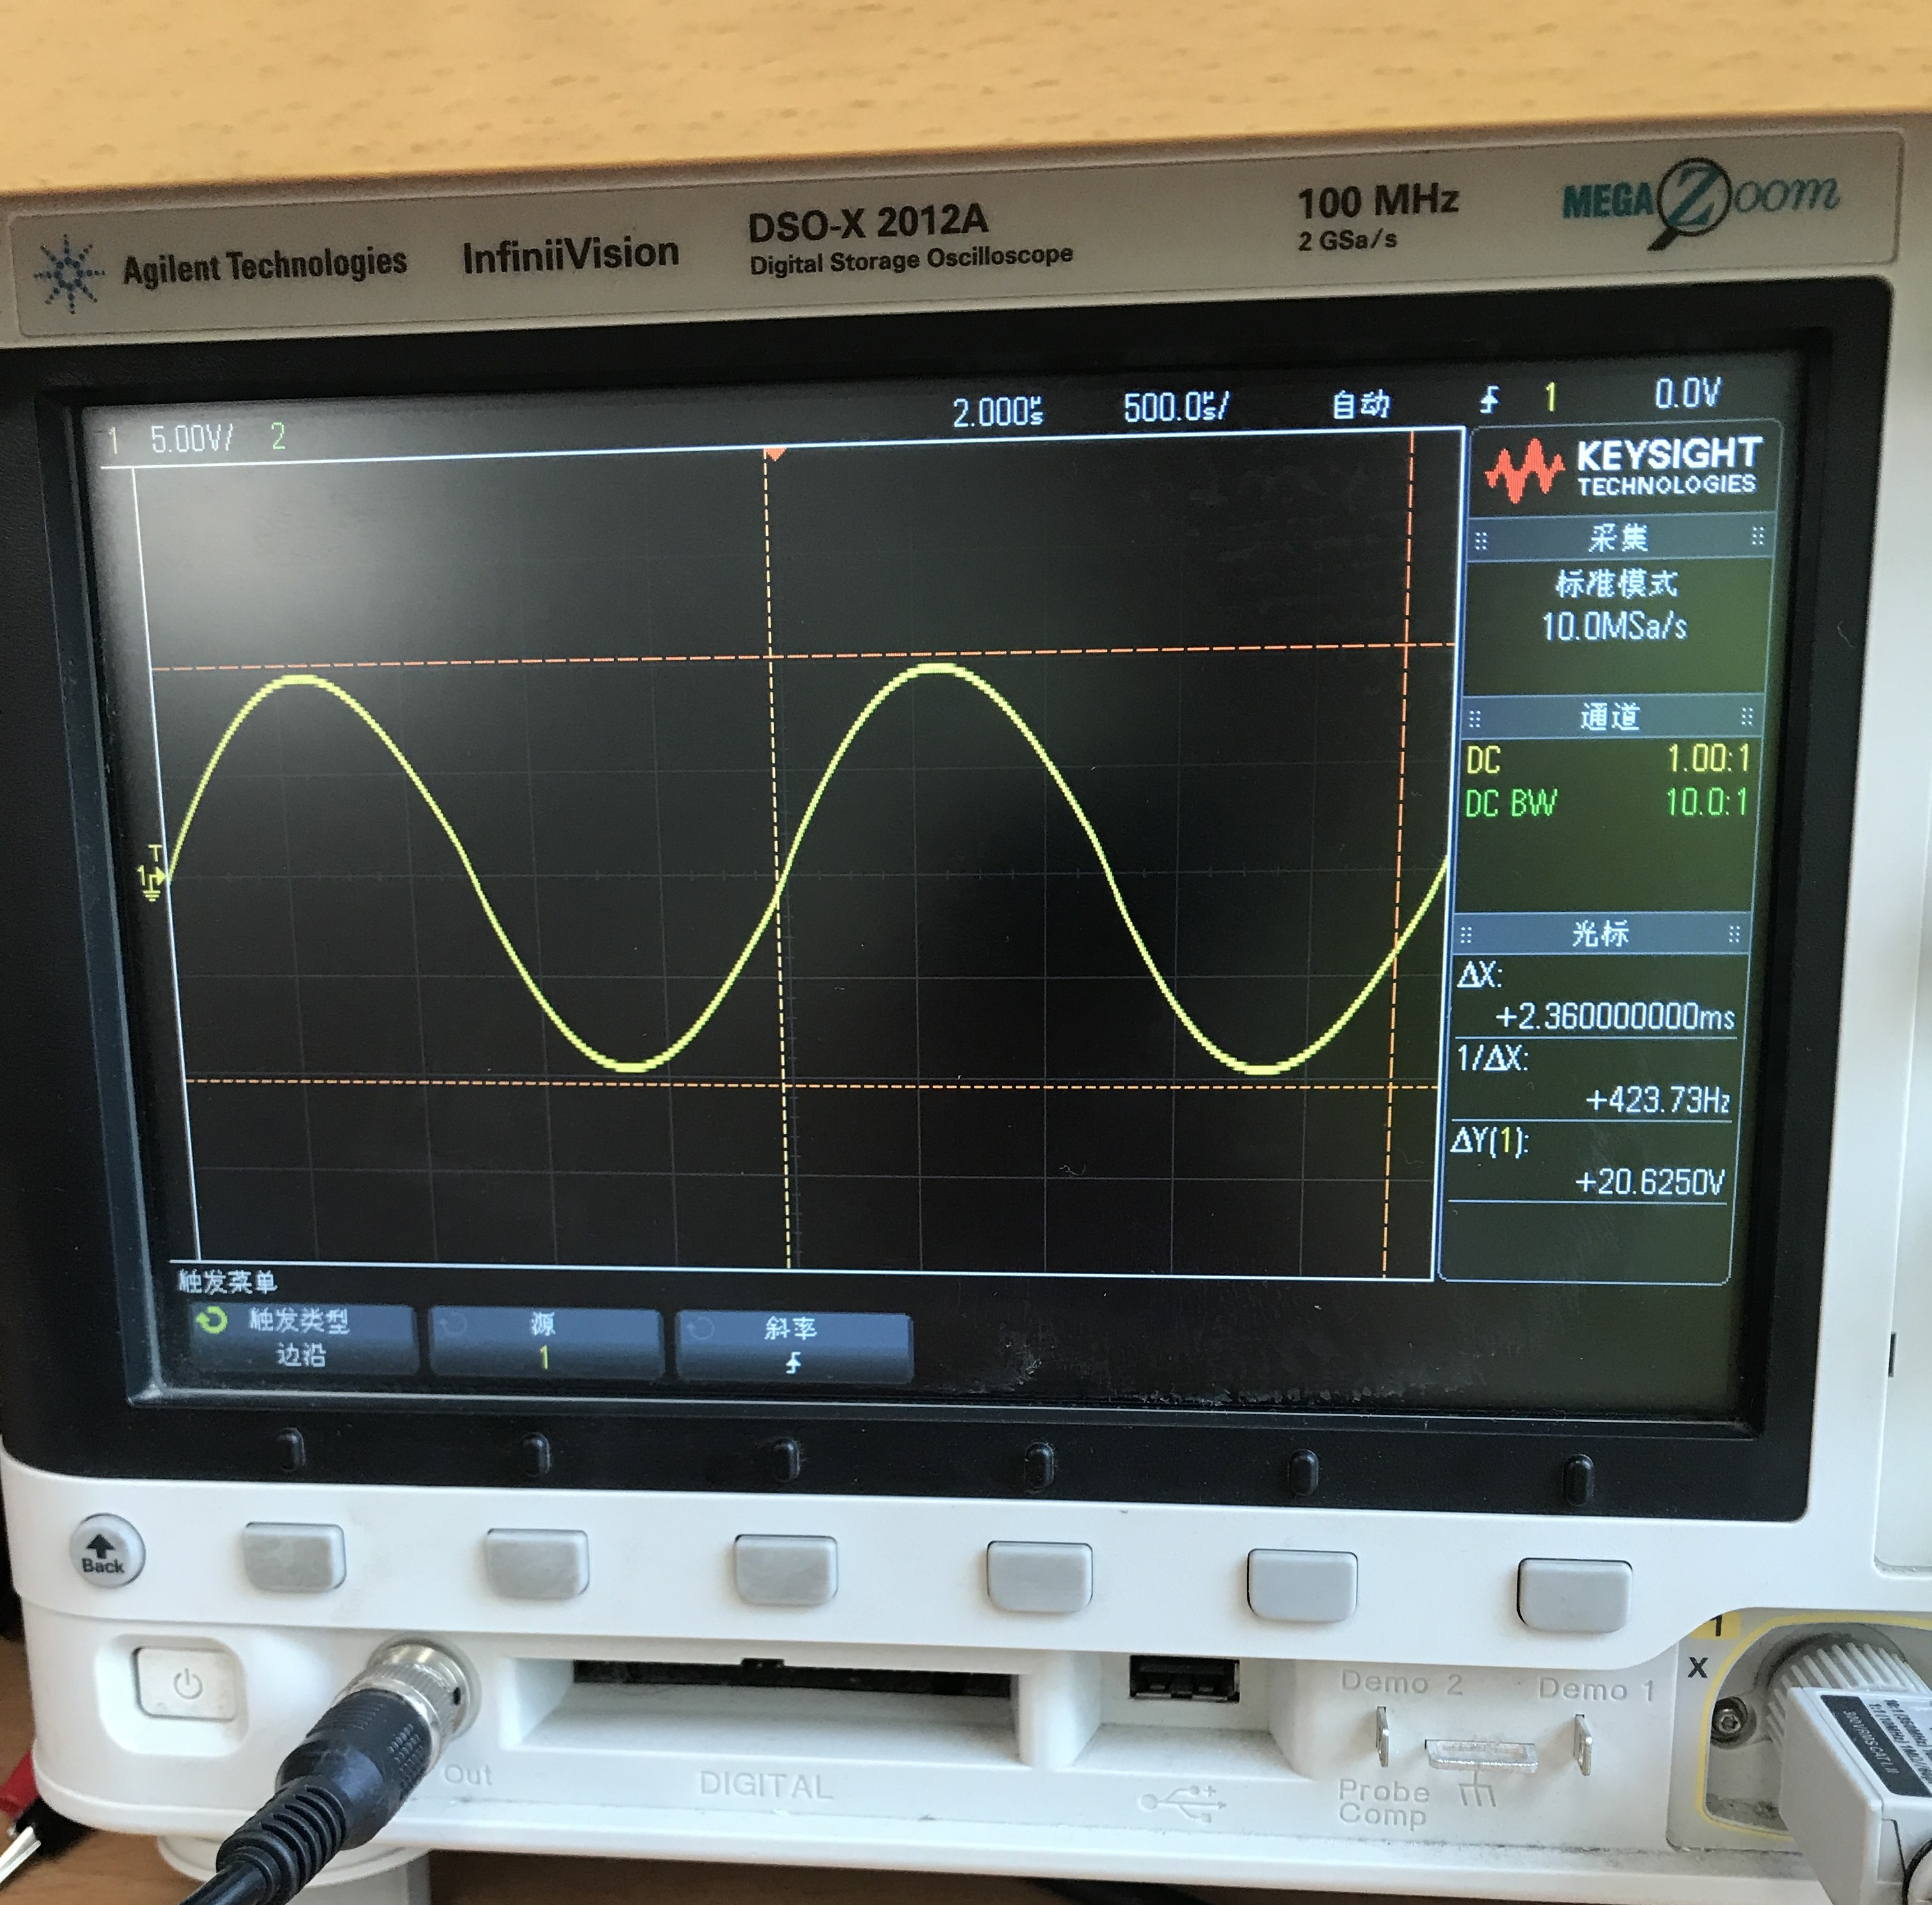
\includegraphics[width=\columnwidth,angle=0]{wave/IMG_0636.jpg}
\caption{最大不失真输出波形}
\label{2}
\end{figure}
\end{multicols}
\begin{multicols}{2}
\subsection{方波——三角波发生电路}
方波发生电路输出电压峰峰值为12V,方波正周期$208\mu\mathrm{s}$,负周期$198\mu\mathrm{s}$,分别对应三角波下降和上升时间,基本对称。三角波峰值为6.4V
\begin{figure}[H]
\centering
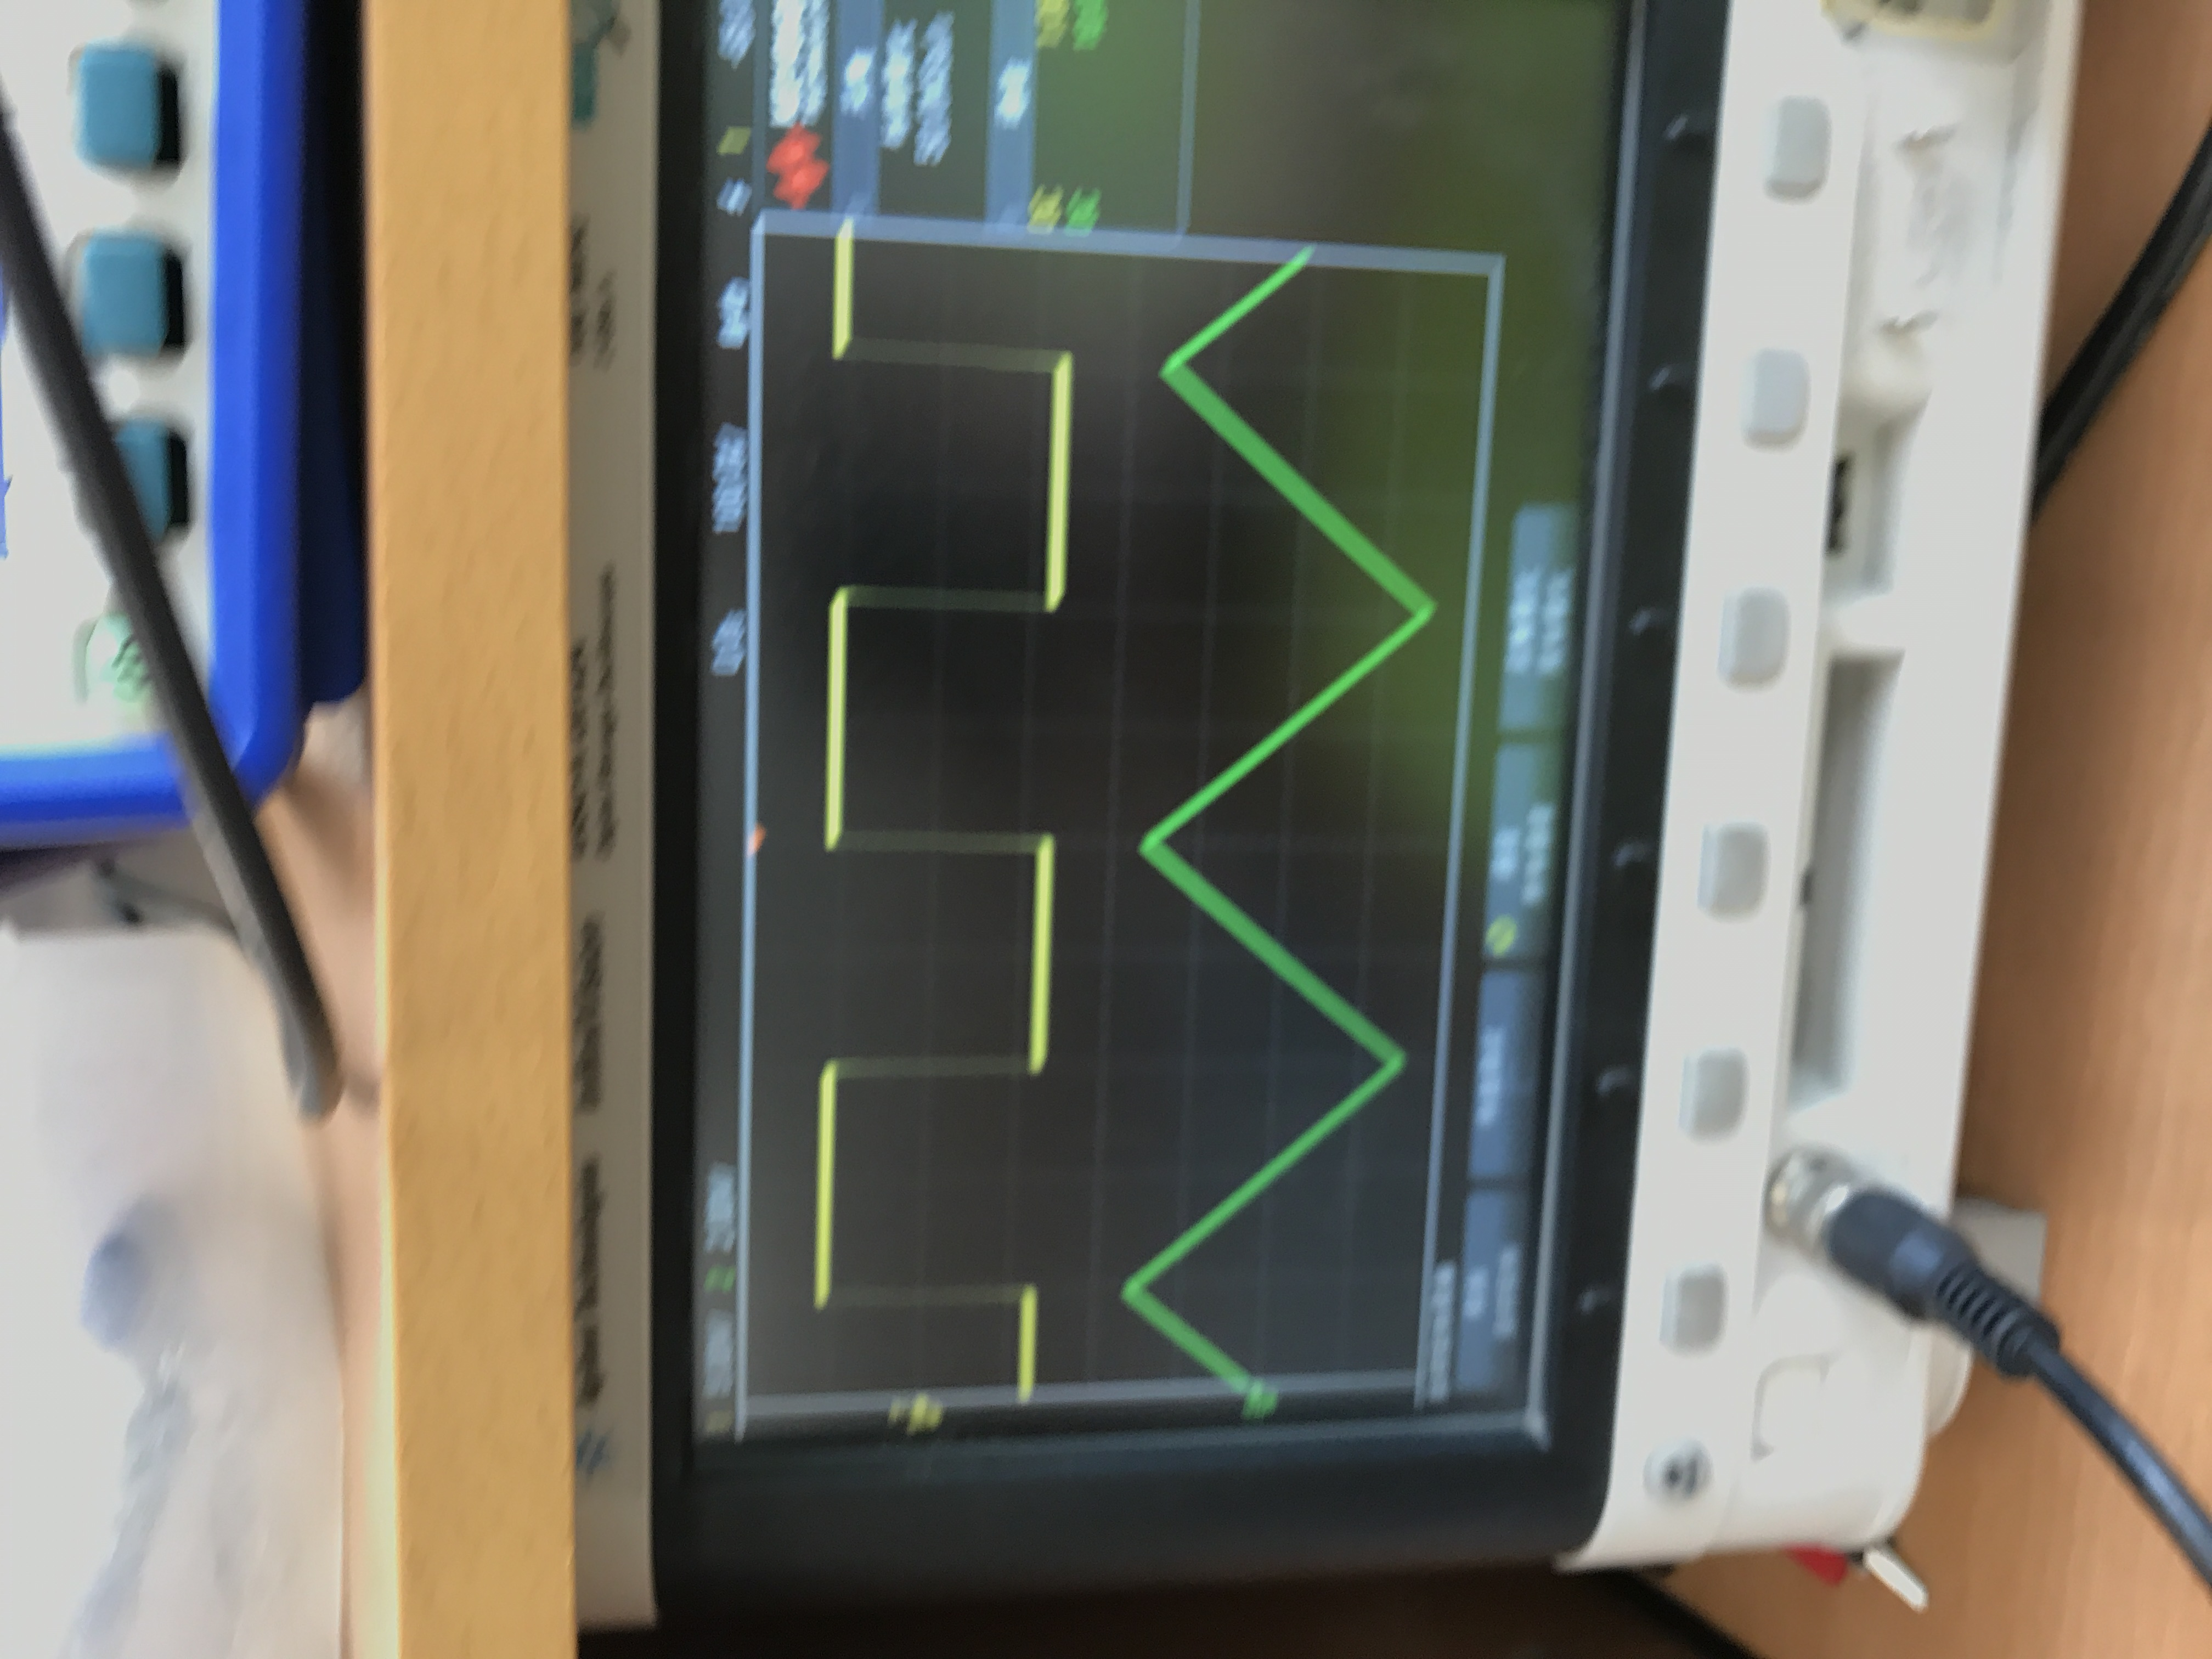
\includegraphics[width=\columnwidth,angle=-90]{wave/IMG_0643.jpg}
\caption{方波输出波形}
\label{3}
\end{figure}
\end{multicols}
\begin{multicols}{2}
\subsection{滞环特性电路的测试}
对滞环特性电路进行调试的过程中发现,电路的正向输出为5.6V,反向输出为-6.1V。$U_{T+}=3.1\mathrm{V},U_{T+}=-2.9\mathrm{V}$
\begin{figure}[H]
\centering
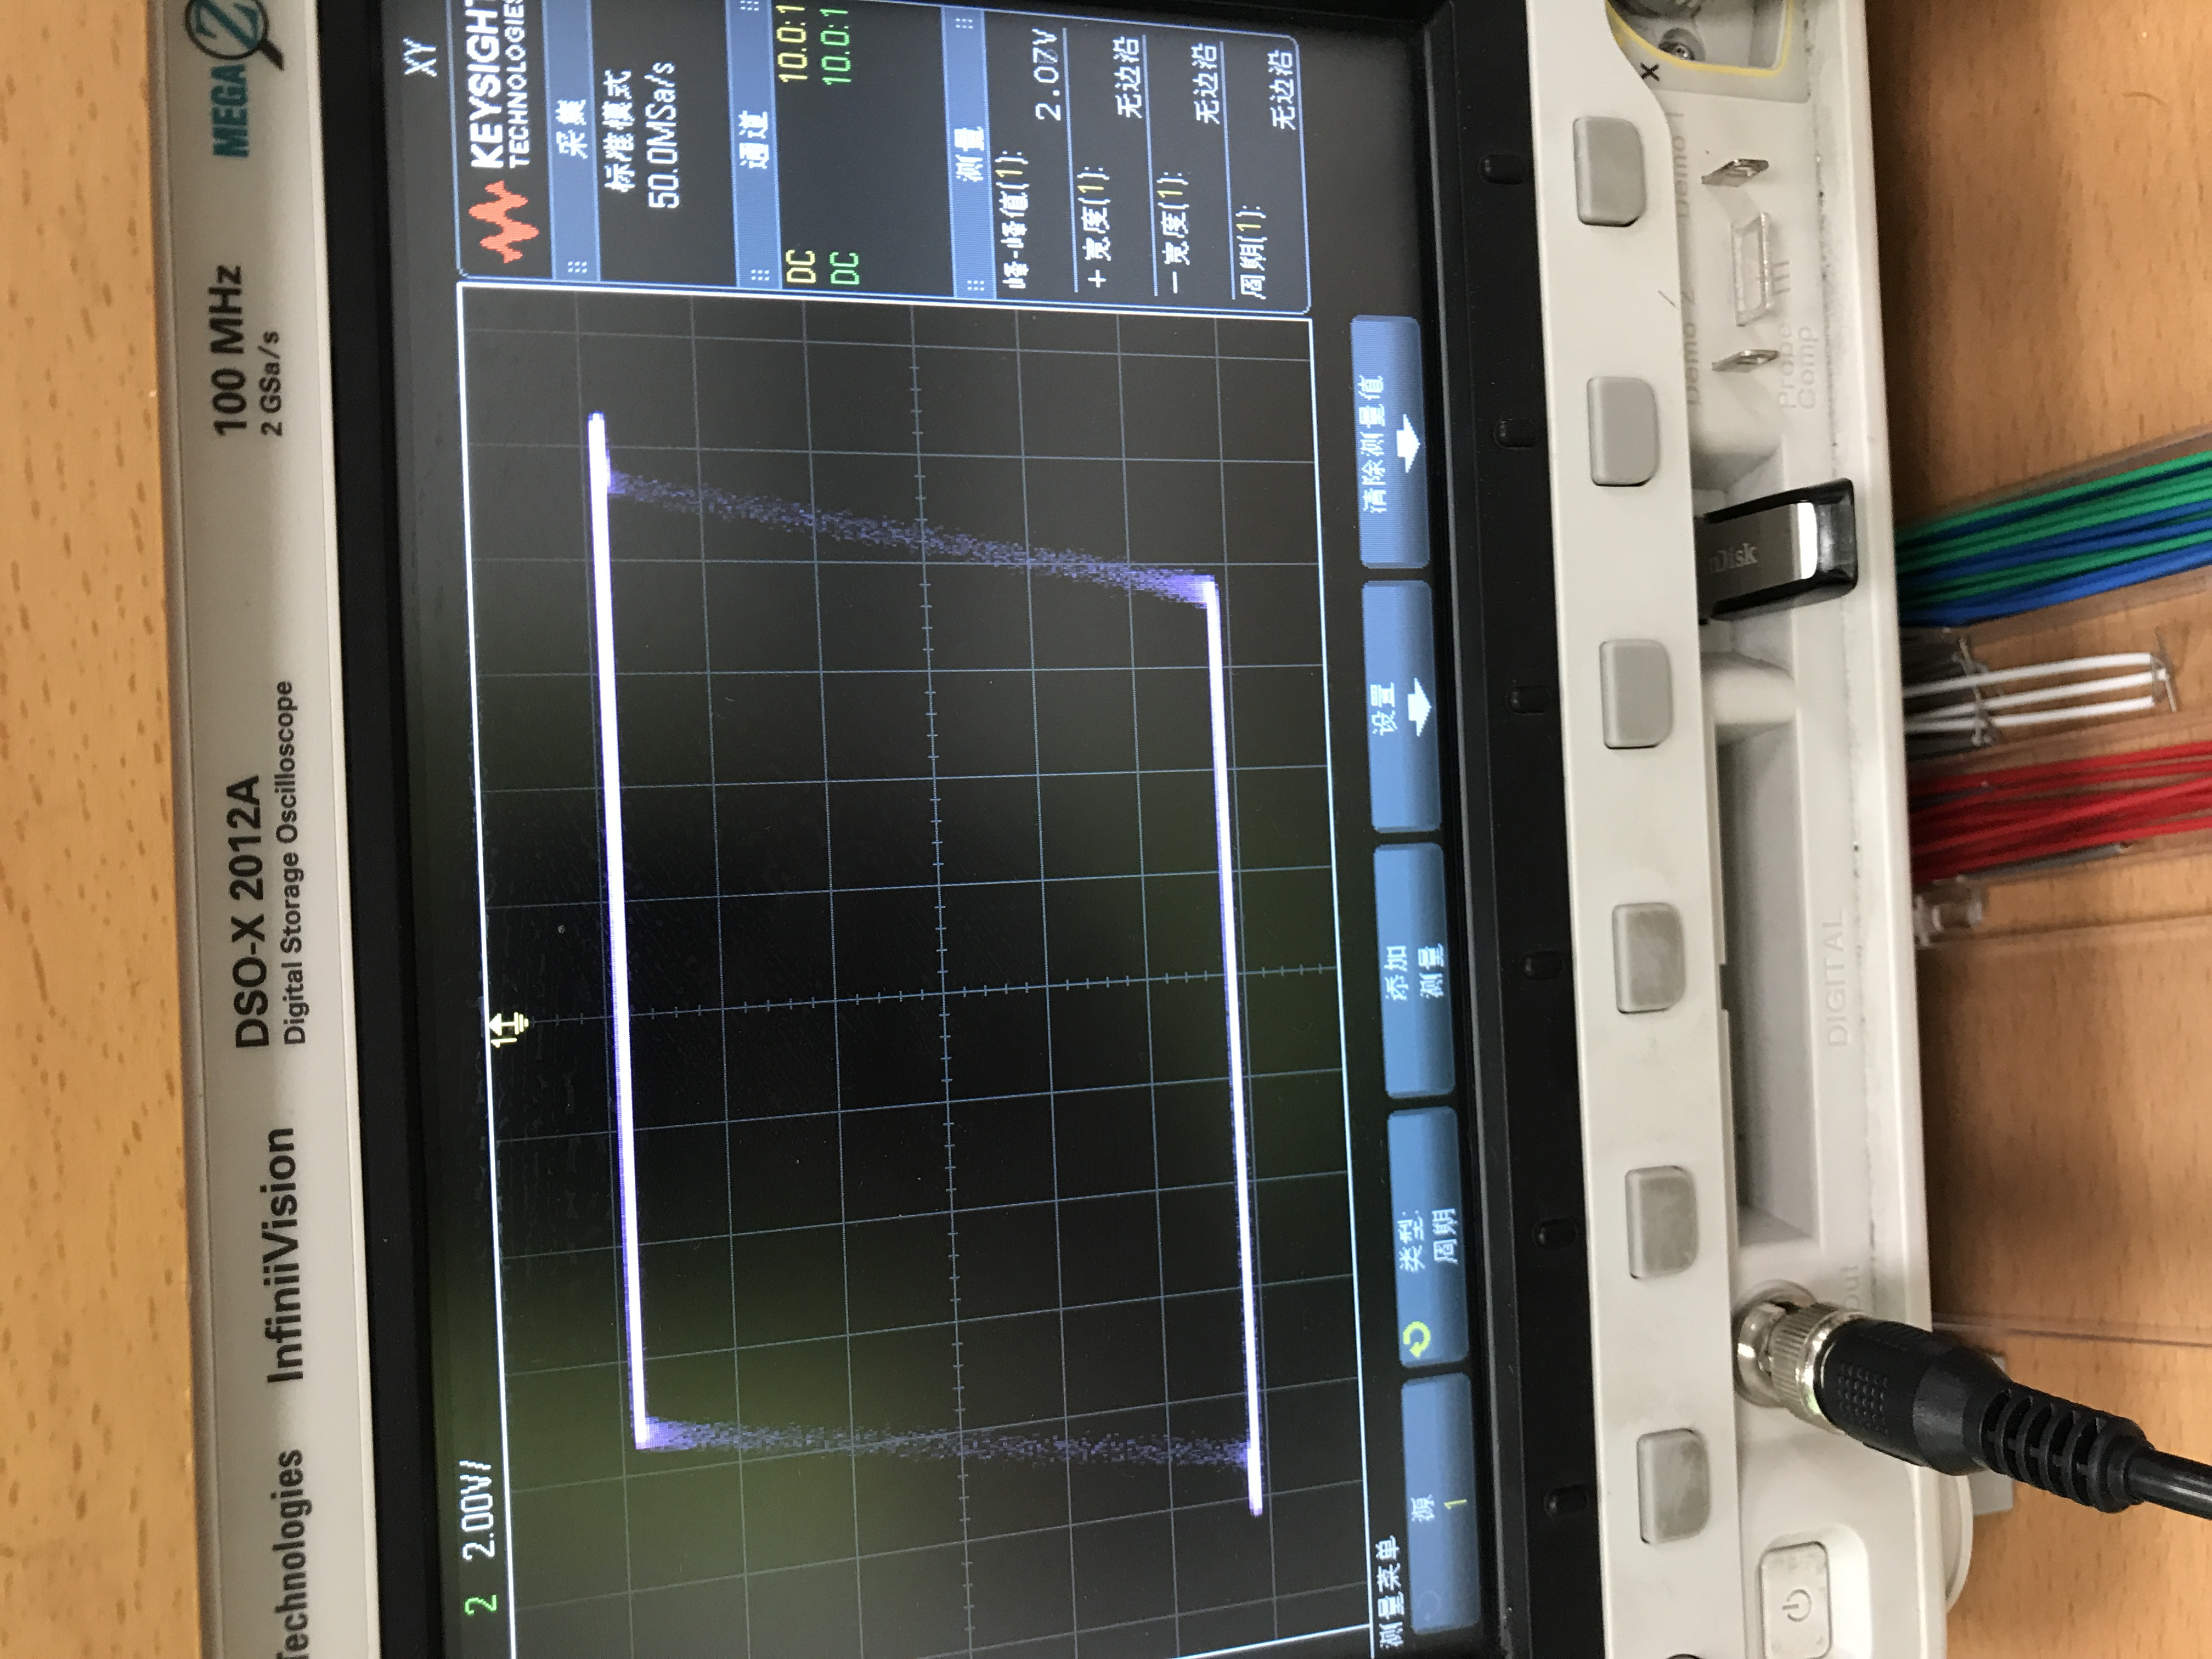
\includegraphics[width=\columnwidth,angle=-90]{wave/IMG_0660.jpg}
\caption{滞环特性输出波形}
\label{4}
\end{figure}
\end{multicols}
\begin{multicols}{2}
\subsection{锯齿波发生电路}
采用$R_1=5.67\mathrm{k}\Omega,R_2=31.2\mathrm{k}\Omega$进行测试(滑动变阻器给出),得到总周期$400\mu\mathrm{s}$,上升时间为$333.33\mu\mathrm{s}$,下降时间为$66.67\mu\mathrm{s}$,正好满足题目要求。
\begin{figure}[H]
\centering
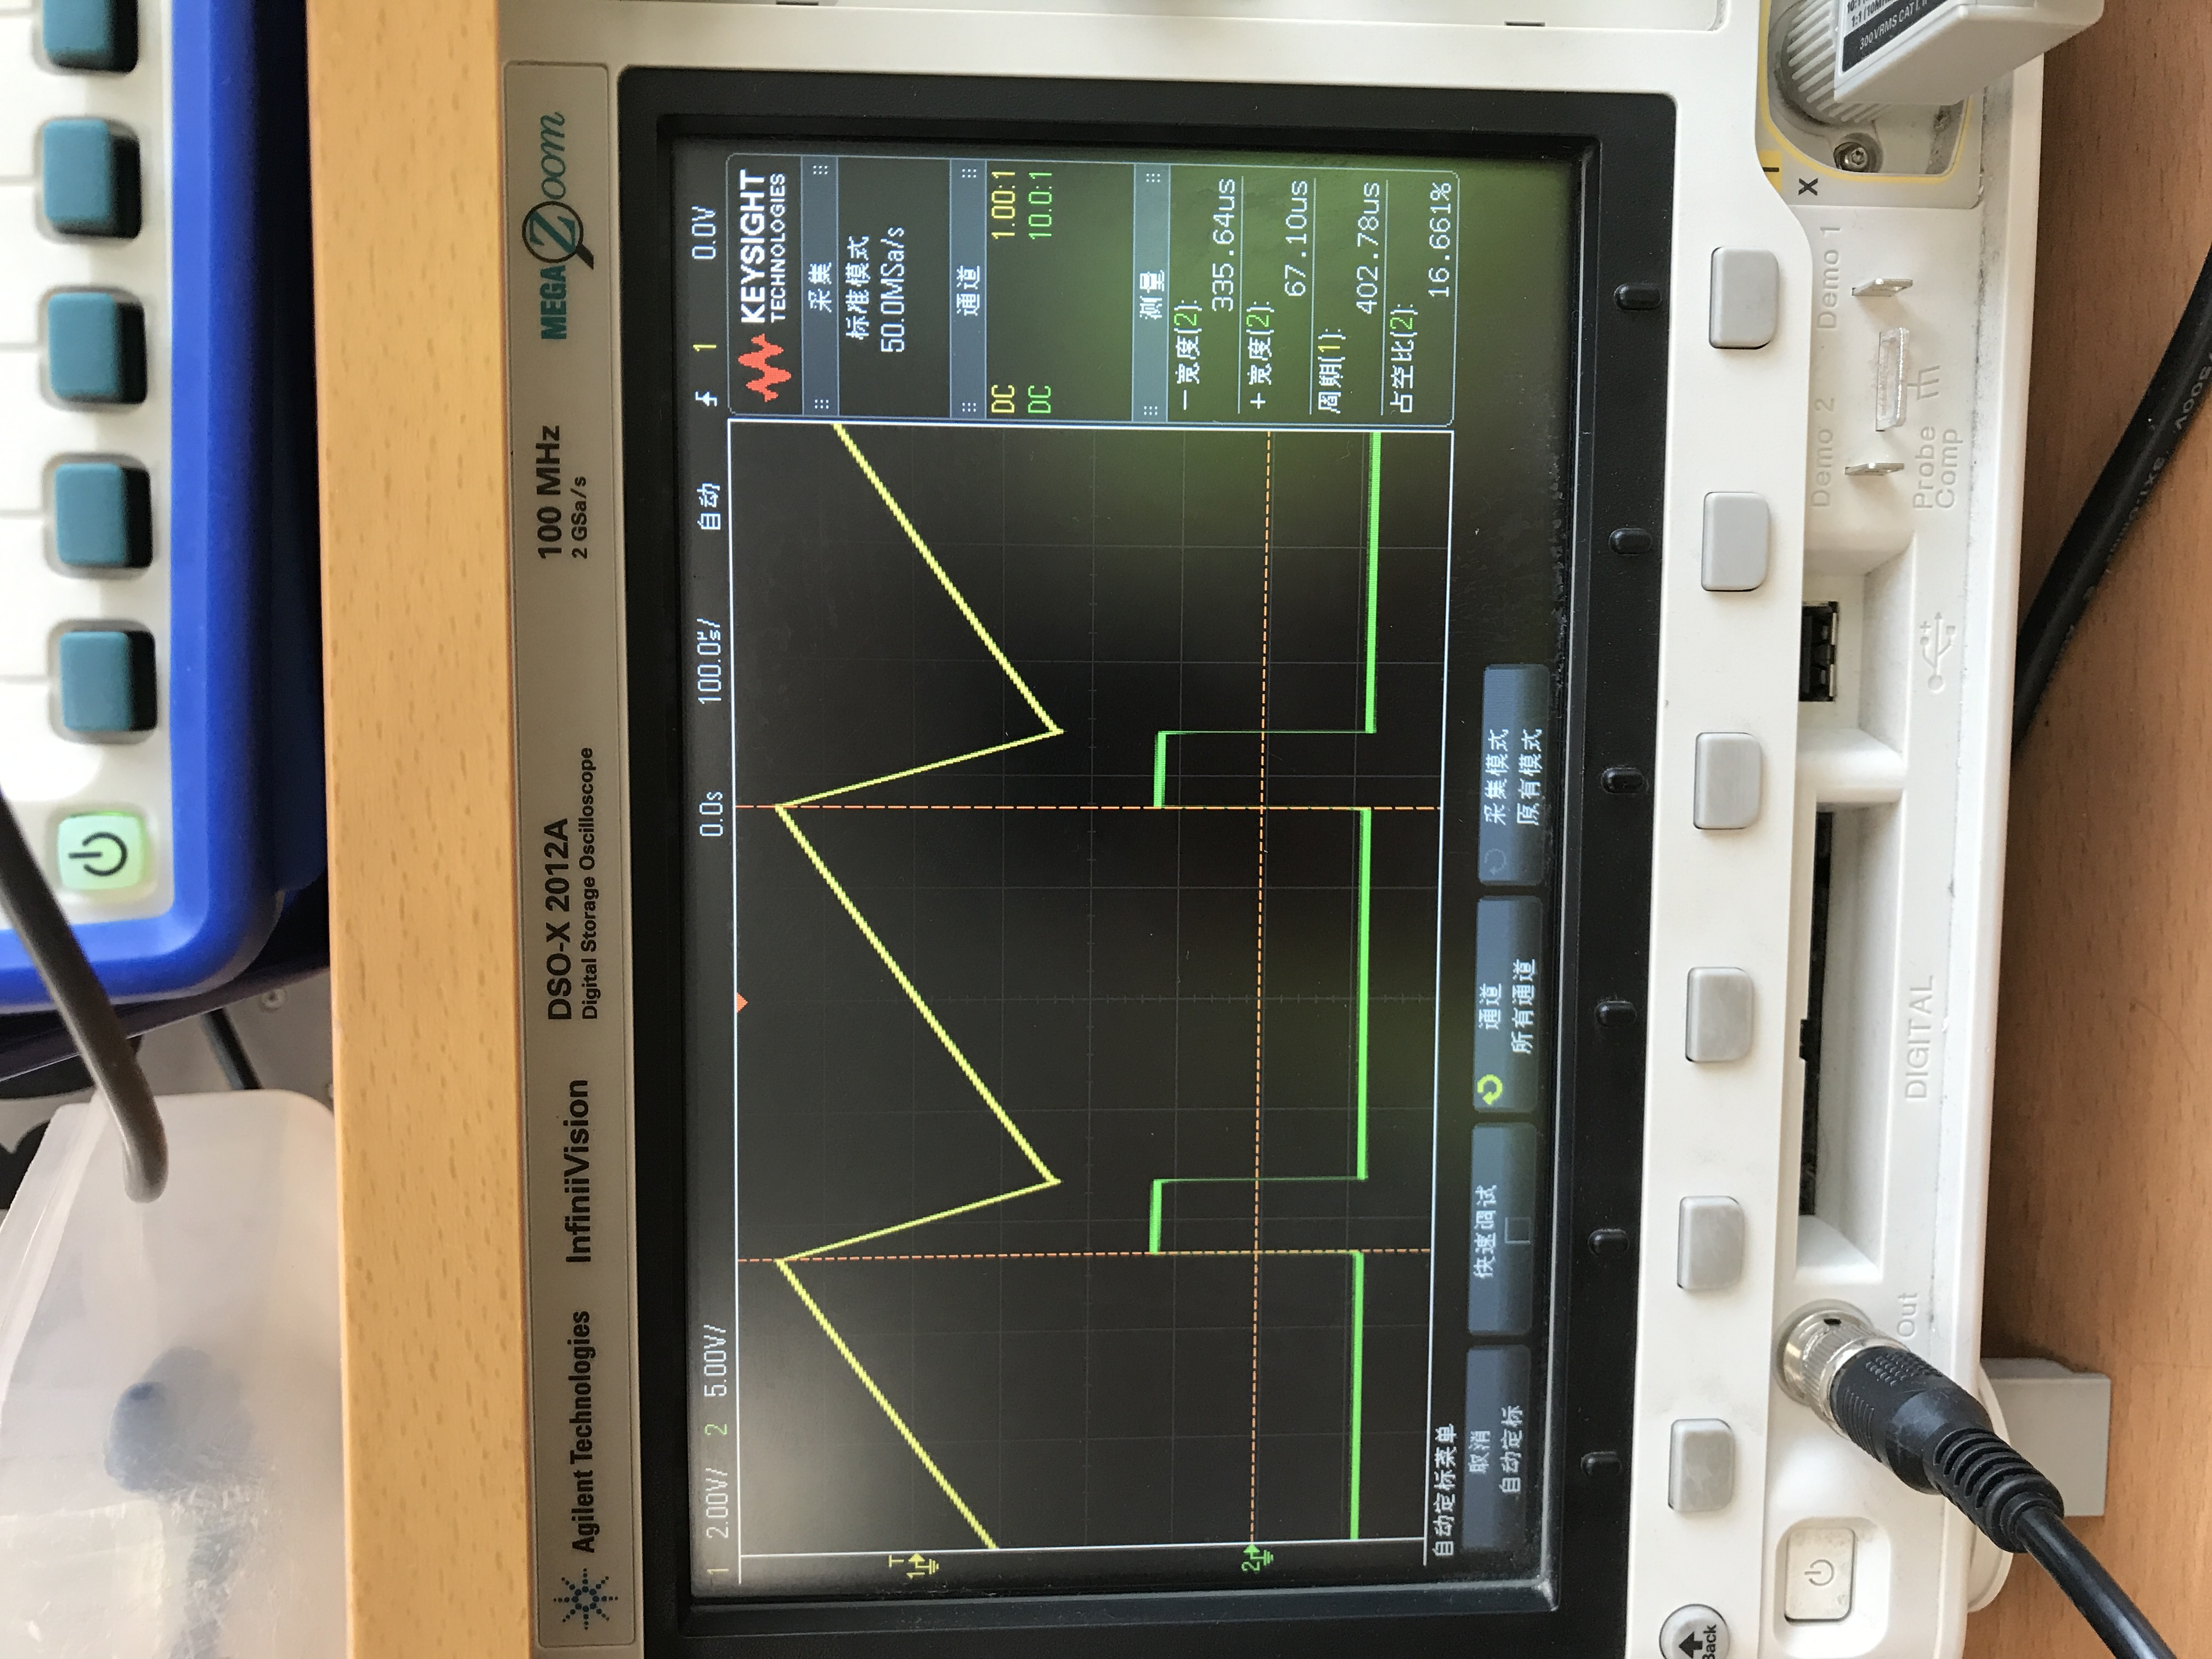
\includegraphics[width=\columnwidth,angle=-90]{wave/IMG_0659.jpg}
\caption{锯齿波输出波形}
\label{5}
\end{figure}
\end{multicols}
\section{总结}
本次实验让我对正弦波,方波,三角波和锯齿波电路更加熟悉,对于波形产生的原理有了一定的了解。在
这个过程中,我更加理解了理论模型、仿真测试和实际电路的联系和区别,并学会分析三者之间产生误差的
原因。

本次试验较为顺利,没有出现电路故障。利用实验室的myDac已经在课前完成了电路的搭建和测试,实验流程非常顺利。
\end{document}